\documentclass[11pt]{article}
\usepackage[utf8]{inputenc}

\usepackage[margin=1in]{geometry}
\usepackage[toc,page]{appendix}
\usepackage{graphicx}
% \usepackage{natbib}
%\usepackage{lipsum}
% \usepackage[style=ieee, citestyle=numeric-comp, backend=biber]{biblatex}
% \usepackage{biblatex}
% \addbibresource{bibliography.bib}
\usepackage{enumerate}
\usepackage{enumitem}
\usepackage{caption}
\usepackage{subcaption}
\usepackage{color}
% \usepackage{hyperref}
\usepackage[pdftex,linkcolor=test,citecolor=vertsombre,colorlinks=true,pagebackref,bookmarks=true, plainpages=true,urlcolor=freeblue]{hyperref}

%%%%%%%%%%%%%%%%%%%%%%%%%%%%%%%%%%%%%%%%%%%%%%%%%%%%%%%%%
%%%%% 	for code
%%%%%
%%%%%%%%%%%%%%%%%%%%%%%%%%%%%%%%%%%%%%%%%%%%%%%%%%%%%%%%%

\usepackage{listings} %for code

\definecolor{codegreen}{rgb}{0,0.6,0}
\definecolor{codegray}{rgb}{0.5,0.5,0.5}
\definecolor{codepurple}{rgb}{0.58,0,0.82}
\definecolor{backcolour}{rgb}{0.95,0.95,0.92}
\lstdefinestyle{mystyle}{
    backgroundcolor=\color{backcolour},   
    commentstyle=\color{codegreen},
    keywordstyle=\color{blue},
    numberstyle=\tiny\color{codegray},
    stringstyle=\color{codepurple},
    basicstyle=\ttfamily\footnotesize,
    breakatwhitespace=false,         
    breaklines=true,                 
    captionpos=b,                    
    keepspaces=true,                 
    numbers=left,                    
    numbersep=5pt,                  
    showspaces=false,                
    showstringspaces=false,
    showtabs=false,                  
    tabsize=2
}
 

\lstset{language=Matlab,%
    %basicstyle=\color{red},
    backgroundcolor=\color{backcolour}
    breaklines=true,%
    morekeywords={matlab2tikz},
    keywordstyle=\color{blue},%
    morekeywords=[2]{1}, keywordstyle=[2]{\color{black}},
    identifierstyle=\color{black},%
    numberstyle=\tiny\color{codegray},
    stringstyle=\color{codepurple},
    commentstyle=\color{green},%
    showstringspaces=false,%without this there will be a symbol in the places where there is a space
    numbers=left,%
    numberstyle={\tiny \color{black}},% size of the numbers
    numbersep=5pt, % this defines how far the numbers are from the text
    emph=[1]{for,end,break},emphstyle=[1]\color{red}, %some words to emphasise
    %emph=[2]{word1,word2}, emphstyle=[2]{style},    
}

\lstset{style=mystyle}
%%%%%%%%%%%%%%%%%%%%%%%%%%%%%%%%%%%%%%%%%%%%%%%%%%%%%%%%%
%%%%% 	pour le français et les accents 	      %%%%%
%%%%%%%%%%%%%%%%%%%%%%%%%%%%%%%%%%%%%%%%%%%%%%%%%%%%%%%%%

\usepackage[T1]{fontenc}
\usepackage[english]{babel}   



      
\usepackage{amsmath}
\usepackage{amssymb}

\usepackage{geometry}
\usepackage{amsthm}       % for theorem definitions
%\usepackage{dsfont}       % for  \mathds and nice 0/1 functions
\usepackage{graphicx}     % for images and graphics
\usepackage{stmaryrd}     % for \llbrackets
%\usepackage{color}
\usepackage{subeqnarray}
%\usepackage{subfigure}


%%%%%%%%%%%%%%%%%%%%%%%%%%%%%%%%%%%%%%%%%%%%%%%%%%%%%%%%%
%%%%% 	police personnelle 	      %%%%%
%%%%%%%%%%%%%%%%%%%%%%%%%%%%%%%%%%%%%%%%%%%%%%%%%%%%%%%%%
\makeatletter
\newcommand\TitleFont{\@setfontsize\Huge{38}{47}} 	%create new font for title



%%%%%%%%%%%%%%%%%%%%%%%%%%%%%%%%%%%%%%%%%%%%%%%%%%%%%%%%%
%%%%% 	Headers and Footers 	      %%%%%
%%%%%%%%%%%%%%%%%%%%%%%%%%%%%%%%%%%%%%%%%%%%%%%%%%%%%%%%%
\usepackage{lastpage}
\usepackage{fancyhdr}
\pagestyle{fancy}
\fancyhf{}
%\cfoot{\small{\thepage/\pageref{LastPage}}}
\renewcommand\headrulewidth{0pt} % Removes header line
\renewcommand\footrulewidth{0.4pt} % Adds footer line

%%%%%%%%%%%%%%%%%%%%%%%%%%%%%%%%%%%%%%%%%%%%%%%%%%%%%%%%%%%
%%%%% 	package pour les algorithmes		       %%%%
%%%%%%%%%%%%%%%%%%%%%%%%%%%%%%%%%%%%%%%%%%%%%%%%%%%%%%%%%%%
\usepackage{algpseudocode}
\usepackage{algorithm}
\usepackage{algpascal}

%%%%%%%%%%%%%%%%%%%%%%%%%%%%%%%%%%%%%%%%%%%%%%%%%%%%%%%%%%%
%%%%% 	pour des liens hypertextes  et du jpg  	      %%%%%
%%%%%%%%%%%%%%%%%%%%%%%%%%%%%%%%%%%%%%%%%%%%%%%%%%%%%%%%%%% 

%%%%%%%%%%%%%%%%%%%%%%%%%%%%%%%%%%%%%%%%%%%%%%%%%%%%%%%%%%%
%%%%%  		Couleurs			%%%%%%%%%%%
%%%%%%%%%%%%%%%%%%%%%%%%%%%%%%%%%%%%%%%%%%%%%%%%%%%%%%%%%%%
%\definecolor{test}{rgb}{0.64,0.16,0.16}
%\definecolor{vertsombre}{rgb}{0.00,0.57,0.1}
%\definecolor{freeblue}{rgb}{0.25,0.41,0.88}

%%%%%%%%%%%%%%%%%%%%%%%%%%%%%%%%%%%%%%%%%%%%%%%%%%%%%%%%%%%




%%%%%%%%%%%%%%%%%%%%%%%%%%%%%%%%%%%%%%%%%%%%%%%%%%%%%%%%%%%
%%%%%%%   	 SHORT CUTS:	  		 %%%%%%%%%%
%%%%%%%%%%%%%%%%%%%%%%%%%%%%%%%%%%%%%%%%%%%%%%%%%%%%%%%%%%%
\newcommand{\nc}{\newcommand}
\nc{\argmin}{\mathop{\mathrm{arg\,min}}}


%%%%%%%%%%%%%%%%%%%%%%%%%%%%%%%%%%%%%%%%%%%%%%%%%%%%%%%%%%%
%%%%%%%  		  SETS:			%%%%%%%%%%%
%%%%%%%%%%%%%%%%%%%%%%%%%%%%%%%%%%%%%%%%%%%%%%%%%%%%%%%%%%%
\def\R{\mathbb{R}}
\def\A{\mathbb{A}}
\def\B{\mathbb{B}}
\def\N{\mathbb{N}}
\def\L{\mathbb{L}}
\def\T{\mathbb{T}}
\def\G{\mathbb{G}}
\def\D{\mathbb{D}}
\def\H{\mathbb{H}}
\def\I{\mathbb{I}}
\def\F{\mathbb{F}}
\def\C{\mathbb{C}}
\def\Z{\mathbb{Z}}


%%%%%%%%%%%%%%%%%%%%%%%%%%%%%%%%%%%%%%%%%%%%%%%%%%%%%%%%%%%
%%%%%%%  		  PROBA			%%%%%%%%%%%
%%%%%%%%%%%%%%%%%%%%%%%%%%%%%%%%%%%%%%%%%%%%%%%%%%%%%%%%%%%
\nc{\ind}{\mathds{1}}
\def\P{\mathbb{P}}
\def\E{\mathbb{E}}
\def\V{\mathbb{V}\mbox{ar}\,}
\def\vt{\mbox{Var}_\theta\,}
\def\cov{\mbox{Cov}\,}
\def\ct{\mbox{Cov}_\theta\,}


%%%%%%%%%%%%%%%%%%%%%%%%%%%%%%%%%%%%%%%%%%%%%%%%%%%%%%%%%%%
%%%%%%%		classe de fonctions		%%%%%%%%%%%
%%%%%%%%%%%%%%%%%%%%%%%%%%%%%%%%%%%%%%%%%%%%%%%%%%%%%%%%%%%
\def\f{{\cal F}} 
\def\g{{\cal G}} 
\def\Lip{\mbox{Lip}\,}


%%%%%%%%%%%%%%%%%%%%%%%%%%%%%%%%%%%%%%%%%%%%%%%%%%%%%%%%%%%
%%%%%%  theorem and others stuffs in English	 %%%%%%%%%%
%%%%%%%%%%%%%%%%%%%%%%%%%%%%%%%%%%%%%%%%%%%%%%%%%%%%%%%%%%%
\newtheorem{theorem}{Théorème}[section]
\newtheorem{lemma}[theorem]{Lemme}
\newtheorem{ex}{Exemple}[section]
\newtheorem{corollary}[theorem]{Corollaire}
\newtheorem{prop}[theorem]{Proposition}
\theoremstyle{remark}
\theoremstyle{definition}
\newtheorem{definition}[theorem]{Définition}
\newtheorem{rem}{Remarque}[section]


%%%%%%%%%%%%%%%%%%%%%%%%%%%%%%%%%%%%%%%%%%%%%%%%%%%%%%%%%%%
%%%%%%  Color for reference links	 %%%%%%%%%%
%%%%%%%%%%%%%%%%%%%%%%%%%%%%%%%%%%%%%%%%%%%%%%%%%%%%%%%%%%%
\usepackage{color}

\usepackage{hyperref}
\hypersetup{
     colorlinks = false
}
%%%%%%%%%%%%%%%%%%%%%%%%%%%%%%%%%%%%%%%%%%%%%%%%%%%%%%%%%%%
%%%%%%  Drawings	 %%%%%%%%%%
%%%%%%%%%%%%%%%%%%%%%%%%%%%%%%%%%%%%%%%%%%%%%%%%%%%%%%%%%%%

%Dessins circuits electroniques
\usepackage[european]{circuitikz}
\usetikzlibrary{babel}

%Pour dessins normaux, contenu dans circuitikz
%\usepackage{tikz}



%%%%%%%%%%%%%%%%%%%%%%%%%%%%%%%%%%%%%%%%%%%%%%%%%%%%%%%%%%%
%%%%%%  Comments	 %%%%%%%%%%
%%%%%%%%%%%%%%%%%%%%%%%%%%%%%%%%%%%%%%%%%%%%%%%%%%%%%%%%%%%

%Commentaires: \begin{comment}...\end{comment}
\usepackage{comment}


%%%%%%%%%%%%%%%%%%%%%%%%%%%%%%%%%%%%%%%%%%%
%%%%%%%%%%% Tikz Utils %%%%%%%
%%%%%%%%%%%%%%%%%%%%%%%%%%%%%%%%%%%%%%%%%%%
\usepackage{tikz}
\def\checkmark{\tikz\fill[scale=0.4](0,.35) -- (.25,0) -- (1,.7) -- (.25,.15) -- cycle;} 
\begin{document}
% \addbibresource{bibliography.bib}
\renewcommand{\headrulewidth}{1pt}
\fancyhead[R]{\today}
\fancyhead[L]{Biomedical Imaging Group}
\renewcommand{\footrulewidth}{1pt}
\fancyfoot[R]{\thepage/\pageref{LastPage}}
\fancyfoot[L]{EPFL}
\setlength{\parskip}{0.7em}

\begin{titlepage}		%Page de titre 
\begin{center} 	


\includegraphics[width=6.5cm]{images/EPFL_Logo.png}	\\[1cm]
\LARGE Project in Microengineering (10 credits)\\ Microengineering Section, Master Semester 4 \\ Spring 2021


\vspace*{\fill}

\Huge {\bfseries Proximal Operators for Nonnegative Inverse Problems }\\[0.5cm]

% \huge {Leg harvesting}\\[1.5cm]
\vspace{20pt}


\LARGE {\emph{Author}}\\ Alejandro Noguerón Arámburu\\ 


\vspace{10pt}

\LARGE {\emph{Supervised by}}\\ Dr. Pol del Aguila Pla \\ 

% \normalsize{\emph{Supervised by:}}  \\
% \large{Niyazi Ulas Dinç}

\vspace{10pt}

\LARGE {\emph{Professor}}\\ Prof. Michael Unser \\ 

% \normalsize{  \emph{Professors} }  \\
% \large{Demetri Psaltis}\\[0.5cm] 	

% \vspace{20pt}

% \large \textit{Section Microtechnique}\\[1cm]

\vspace*{\fill}

\today
\end{center}
\end{titlepage}



%%%%% Beginning of the document

\setcounter{page}{0}
\fancyfoot[C]{\thepage}


% \input{0_Summary}
%attention aux espaces
%\renewcommand\thesection{\Roman{section}}
%\renewcommand\thesubsection{\thesection. \Alph{subsection}}
%\renewcommand\thesubsubsection{\thesubsection. \arabic{subsubsection}}


\newpage
\tableofcontents

\newpage
\section{Introduction} \label{sect:1}

The present semester project has the aim of exploring properties of the proximal operators of common image regularizers -used to promote a desirable property like sparsity or smoothness in reconstructed images-, which play a critical role in image reconstruction across different fields of science, engineering and medicine. I will study their behaviour when they are combined with nonnegativity constraints, a term that will penalize the reconstruction infinitely when there is any negative term in the result. This is of particular importance because in scientific imaging, images are formed from physical signals constrained to a known range. Specifically, for a given regularizer $\mathcal{R}: \mathbb{R}^N\rightarrow \mathbb{R}$ we want to test whether
\begin{equation}
\begin{split}
        \mathrm{prox}_{\mathcal{R} + \delta_{\rm \mathbb{R}_+^N}}(\mathbf{v}) &= \mathrm{prox}_{\mathcal{R}}(\mathrm{prox}_{\delta_{\rm \mathbb{R}_+^N}}(\mathbf{v}))\mbox{, or}\\
        \mathrm{prox}_{\mathcal{R} + \delta_{\rm \mathbb{R}_+^N}}(\mathbf{v}) &= \mathrm{prox}_{\delta_{\rm \mathbb{R}_+^N}}(\mathrm{prox}_{\mathcal{R}}(\mathbf{v})).
    \end{split}    
\end{equation}
Any of the two fulfilled conditions can potentially %enable reduced splitting -necessary for the current algorithm of choice, ADMM (see section \ref{sect:1.prox})-, therefore 
improve computational performance when using proximal optimization algorithms for image reconstruction.

In this section I will describe the general imaging problem, which is recovering a representation of an object from noisy measurements. Furthermore, I will describe how optimization and regularization play a key role in solving it. In Section \ref{sect:2}, I will describe some relevant image regularizers, along with the concept of proximal operator and its applicability in image reconstruction problems. Moreover, I will present some examples of optimization algorithms that rely on the proximal operator. In Section \ref{sect:2_methods} I will give a description of the methods and the computational environment I used throughout the project. Finally, in Section \ref{sect:3}, I will present and discuss the results of the project.  



% Throughout this section, in \label{sect:1.imaging}, I will first describe the general imaging problem, that is, recovering a representation of an object from noisy measurements, and how regularization and optimization play a key role in solving it. In section \ref{sect:2} I will describe the most common image regularizers, as well as the concept of proximal operator and its link to the most common algorithms to solve image reconstruction problems, as well as the most representative of these algorithms for out purposes. In section \ref{sect:2environment} I will give a description of the methods I used throughout the project, and finally, in section \ref{sect:3} I will present the results of this work.

\subsection{Imaging as an Inverse Problem} \label{sect:1.imaging}

An imaging problem \cite{soubies_pocket_2019, noauthor_tutorial_2020} takes the form
\begin{equation}
    \mathbf{y} = \mathbf{Hx} + \mathbf{w}\mathrm{,}
    \label{eq:imaging_compact}
\end{equation}
where $\mathbf{y} \in \mathbb{R}^M$ corresponds to discrete measurements recorded by an imaging system, and $\mathbf{x}\in \mathbb{R}^N$ is the representation of a \textit{d}-dimensional, continuously defined object. $\mathbf{x}$ and $\mathbf{y}$ are therefore related through the linear operator $\mathbf{H}:\mathbb{R}^N\rightarrow\mathbb{R}^M$ that models the imaging system (for example, the Radon transform in the case of computer tomography). Then, $\mathbf{Hx}$ corresponds to a noiseless representation that reaches a detector with the added noise $\mathbf{w} \in \mathbb{R}^M$. The noise $\mathbf{w}$ is assumed to be independent and identically distributed (i.i.d.), and it is usually modelled as Gaussian. 

Therefore, the imaging task consists of recovering $\mathbf{x}$ from the measurement $\mathbf{y}$. The \textit{forward} model is given by $\mathbf{H}$ (it is assumed to be known, at least up to some variation), and the problem of recovering $\mathbf{y}$ is referred to as an \textit{inverse} problem. 

The most immediate solution is to solve the \textit{least squares} optimization problem
\begin{equation}
    \arg \min_{\mathbf{x}\in \rm \mathbb{R}^N}\|\mathbf{Hx} - \mathbf{y}\|^2_2
    \label{eq:least_squares}
\end{equation}
Which makes $\mathbf{Hx}$ as similar to $\mathbf{y}$ as possible, where $\mathbf{x}$ is an optimization variable whose optimal value should be a representation of the original object. Note that, since $\mathbf{H}$ is known, a value of $0$ for this objective is equivalent to having a noiseless measurement. Given that the noise is assumed to be i.i.d, solving \eqref{eq:least_squares} is corresponds to using the maximum likelihood estimation. 

The solution $\mathbf{\hat{x}}_\mathrm{LS}$ to the least squares problem is available in closed-form as
\begin{equation}
    \mathbf{\hat{x}}_\mathrm{LS} = (\mathbf{H}^T\mathbf{H})\mathbf{H}^T\mathbf{y}\mathrm{.}
    \label{eq:least_squares_solution}
\end{equation}
However, inverse problems are generally ill-posed, which means, among other things, that there are many solutions  $\mathbf{\hat{\mathbf{x}}}_\mathrm{i}$ for which $\mathbf{\hat{\mathbf{x}}}_1 = \mathbf{\hat{x}}_2$ yields $\mathbf{H}\mathbf{\hat{x}}_1 = \mathbf{H}\mathbf{\hat{x}}_2$, and this often results in non-desirable artifacts. Moreover there is no guarantee that $\mathbf{\hat{x}}_\mathrm{LS}$ will be similar to the true $\mathbf{x}$. To \textit{guide} the solution, it is necessary to include previous knowledge about the object in  $\mathbf{x}$. For the scope of this project, we will look at two terms that can be added to the minimization objective of \eqref{eq:least_squares}. 

The first additional term is used to restrict the solution to nonnegative elements, and it is given by
\begin{equation}
    \delta_{\rm \mathbb{R}_+^N}(\mathbf{x}) =
    \begin{cases}
        \begin{split}
        0\qquad \mbox{if } &\mathbf{x} \in \rm \mathbb{R}_+^N\mathrm{,} \\
        + \infty \ \mbox{   if } &\mathbf{x}\, \notin \rm \mathbb{R}_+^N\mathrm{.}
        \end{split}
     \end{cases}
    \label{eq:indicator_function}
\end{equation}
Here, $\delta: \mathbb{R}^N \rightarrow \mathbb{R}_+ \bigcup \{+\infty\}$ is an indicator function that forces the solution into a particular set, in this case, the set of nonnegative vectors $\mathbb{R}_+^\mathrm{N}$. Since the values are limited to $\{0, \infty\}$, this term guarantees that the solution will not have any nonnegative element, as the value of the objective function go to $\infty$. On the other hand, inside the valid set, it will have no further effect. 

The second term that is added to the objective function is given by:
\begin{equation}
        \mathcal{R}(\mathbf{x}) = \operatorname{R}(\mathbf{Lx})
    \label{eq:regularizer}
\end{equation}
In  \eqref{eq:regularizer}, $\mathcal{R}: \mathbb{R}^N \rightarrow \mathbb{R}$ is an operator that \textit{measures} a transform $\mathbf{L}: \mathbb{R}^N \rightarrow \mathbb{R}^Q$ of $\mathbf{x}$ through the scalar function $\operatorname{R}: \mathbb{R}^Q \rightarrow \mathbb{R}$. Thus, $\mathcal{R}$ is a scalar quantity that represents a property of $\mathbf{x}$ that is desired to be small. In the case of imaging problems, previous knowledge can often be encoded as sparsity, either directly on $\mathbf{x}$ (the case in which $\mathbf{L} = \mathbf{I}$) or on a transform $\mathbf{Lx}$. Thus, a common choice for $\operatorname{R}$ is the $\ell_1$ norm, but there are many sophisticated choices (see Section \ref{sect:2regularizers} for more details). 

Finally, it is important to say that while it is necessary to have a measure of similarity between $\mathbf{Hx}$ and $\mathbf{y}$, the sum of squares is by no means the only choice. Thus, we will denote the measure of similarity between forward model and measurements by $\mathcal{D}(\mathbf{Hx}, \mathbf{y})$, where $\mathcal{D}: \mathbb{R}^M \times \mathbb{R}^M \rightarrow \mathbb{R}$. However, the choice of $\mathcal{D}$ is outside of the scope of this project. 

With that, we arrive at the most common optimization problem in imaging,
\begin{equation}
    \arg \min_{\mathbf{x}\in\mathbb{R}}\mathcal{D}(\mathbf{Hx}, \mathbf{y}) +  \mathcal{R}(\mathbf{Lx}) + \delta_{\mathbb{R}_+^\mathrm{N}}(\mathbf{x}).
    \label{eq:imaging_problem}
\end{equation}
This minimization problem -evidently more complex than the one presented in  \eqref{eq:least_squares}- has several difficulties. One of them is that there is no closed form solution as in \eqref{eq:least_squares}, so the solution has to be found through iterative algorithms. These algorithms usually require first-order information (e.g. the gradient) or second-order information (e.g. the Hessian, which is used in iterative algorithms to achieve faster convergence). However, biomedical imaging has the constraint that even if second derivatives are available, the size of $\nabla^2f(\mathbf{x}) \in \mathbb{R}^{N^2}$ is the squared of the size of $\mathbf{x}$. In an image of $256\times 256$ pixels, this is in the order of $10^{10}$, which means that it cannot be easily stored. Thus, there is a need to restrict to first-order methods, otherwise the computational memory requirements are simply too high. Moreover, image regularizers in general are or include norms, which are non-smooth and non-differentiable, whilst the nonnegativity constraint is highly non-smooth. Therefore, the optimization problem \eqref{eq:imaging_problem} is not solvable through algorithms designed for smooth optimization like gradient descent, and proximal algorithms are required. 

To solve the objective function, algorithms like the alternating direction method of multipliers (ADMM) are used. ADMM is a common and representative example of an iterative algorithm that can solve the optimization problem \eqref{eq:imaging_problem}, but there are several options. ADMM performs one splitting per term in the objective function, and solves its proximal operator, a process that is guaranteed to converge but increments the computational cost and memory requirements for each split. Thus, investigating the proximal operator of common regularizers in combination with nonnegativity constraints could provide significant speed-ups and memory savings in image reconstruction tasks. % In section 2 I will first deepen on the topic of common image regularizers. Then, I will explain the proximal operator and its related optimization algorithms, as well as the closed form solutions for the proximal operator of functions of interest. 


% % \newpage
\section{Background} \label{sect:2}

In this Section~I will deepen on the theoretical background required for the project. First, in Section~\ref{sect:2regularizers}, I will describe $\ell_1$ and $\ell_2$ norm regularization and common image regularizers like total variation ($\operatorname{TV}$), group sparsity and the Hessian-Schatten norm. Then, in Section~\ref{sect:2prox}, I will describe the proximal operator and some relevant optimization algorithms for image reconstruction. 

\subsection{Image Regularization}  \label{sect:2regularizers}

As mentioned in Section~\ref{sect:1}, sparsity is a well known property of real life images and objects. In particular, sparsity on transforms that measure variation in the vicinity of pixels (e.g., the wavelet transform \cite{vonesch_fast_2009}, or derivative operators \cite{soubies_pocket_2019, chambolle_image_1997}) promote smoothness on an image, and in many cases they are a good indicator of low noise and high fidelity with the true object. Moreover, the $\ell_1$ norm is a good objective function to promote sparsity, which is why common image regularizers are a combination of $\ell_1$ norms measuring a transform $\mathbf{L}$ that measures a property that is desired to be small.

Other desirable properties in image regularizers are convexity -to make optimization feasible- and  invariance to rotation, translation, and scaling, so that they do not depend on any specific coordinate axis. 

\noindent\textbf{$\mathbf{\ell_p}$ regularization} 

As aforementioned, $\ell_1$ and $\ell_2$ norms are common choices of $\operatorname{R}$ for regularization. When acting on a raw measurement, $\ell_p$ regularization consists in choosing the point within a validity region (which can be determined by a scaling parameter $\lambda$ multiplying $\mathcal{R}$ in \eqref{eq:imaging_problem}) that touches the smallest norm ball of the chosen $\ell_p$ norm. This is exemplified in Figure \ref{fig:l1_reg} (reused with permission from \cite{noauthor_tutorial_2020}) for the $\ell_1$ and $\ell_2$ norms.  
\begin{figure}[H]
  \begin{center}
  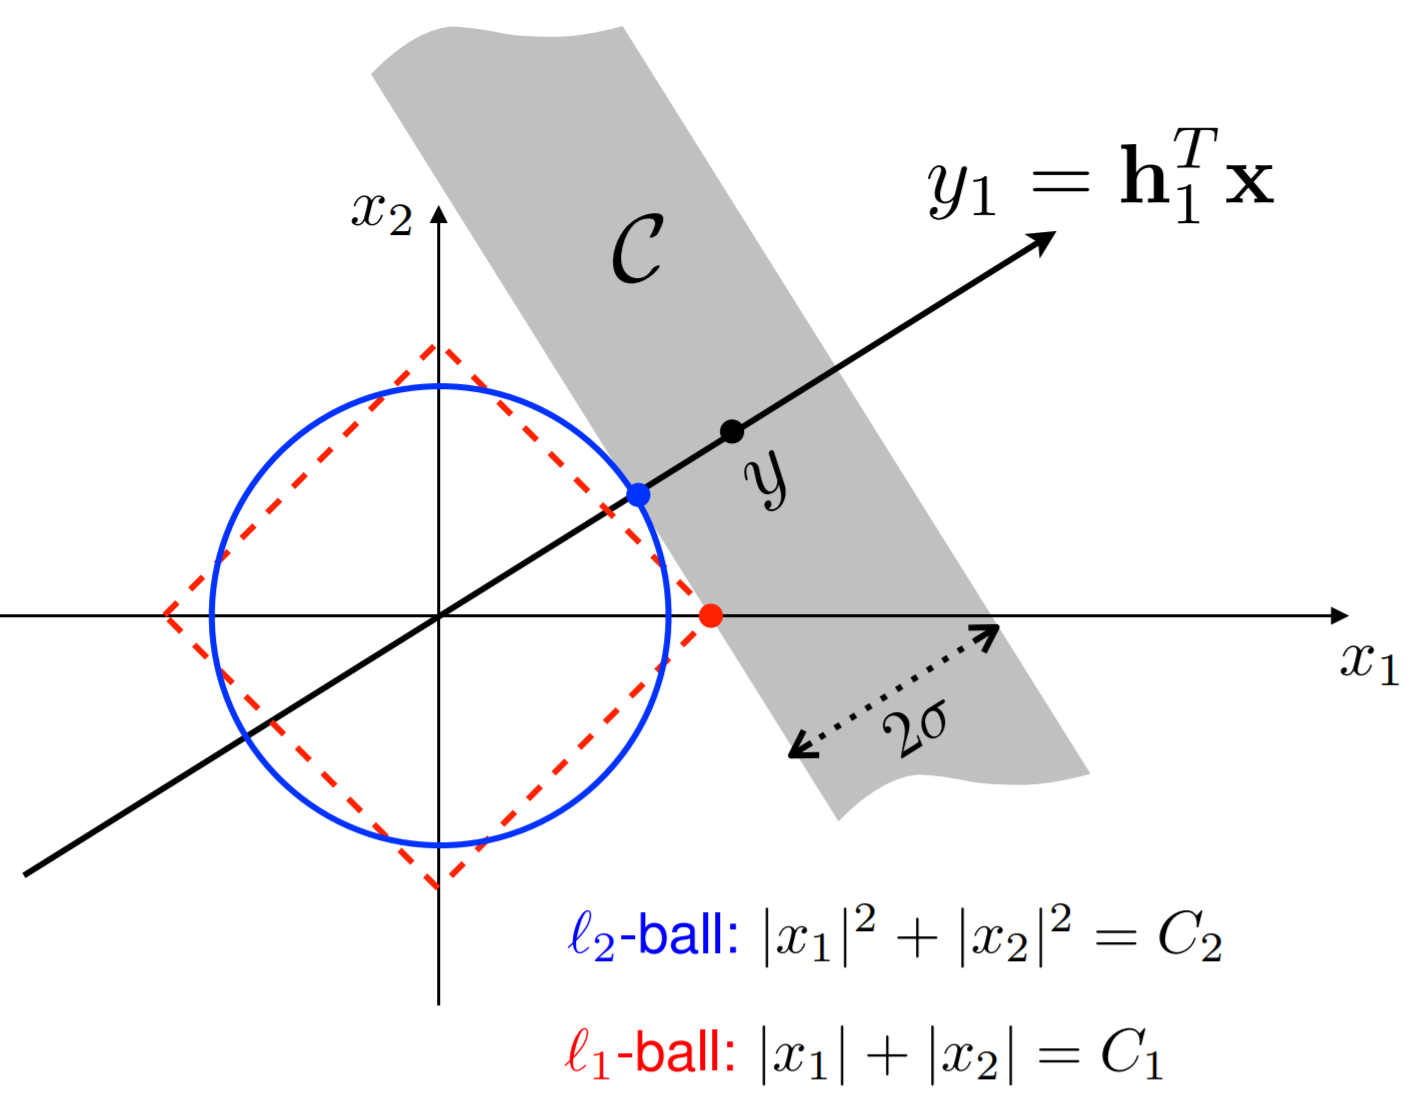
\includegraphics[width = 0.55
  \textwidth]{images/l1_reg.PNG}
  \caption{$\ell_1$ and $\ell_2$ norm regularization on a low dimensional example. The regularization of $\mathbf{x}$ consists in finding the points (in red for the $\ell_1$ norm and blue for the $\ell_2$ norm) as optimal reconstruction. The gray area corresponds to the data fidelity region. Figure reused with permission from \cite{noauthor_tutorial_2020}.}
  %$y_1$ (obtained from the sampling $\mathbf{h}_1^T\mathbf{x}$) results in choosing the points $x_1$ and $x_2$ within the data fidelity region (shaded in gray) that touch the smallest possible norm balls within this region. Figure taken from \cite{noauthor_tutorial_2020}.} 
  \label{fig:l1_reg}
  \end{center}
\end{figure}

In Figure \ref{fig:l1_reg}, in an example of a $2$-dimensional inverse problem, the properties of $\ell_1$ and $\ell_2$ regularization are exemplified. The solution of $\ell_2$ norm regularization lies within the space spanned by $\mathbf{h}_1^T$, but does not necessarily promote sparsity. On the other hand, $\ell_1$ regularization promotes sparsity in the solution -under some conditions in $\mathbf{h}_1^T$-.

\noindent\textbf{Group Sparsity}

In images where there is prior information on the structure of the image in the form of pixel labelling (e.g., many cell images where structural information can be known \cite{baritaux_sparsity-driven_2011}, or using a spatio-temporal representation of a single image \cite{del_aguila_pla_cell_2018-1, del_aguila_pla_cell_2018}), $\ell_p$ norm regularization can be applied independently (without overlap) to the different structures. This results in a vector of measurements of each region, and a second norm can be taken over this new vector. This technique has been proven to be successful in image reconstruction tasks, and is known as group sparsity. It is also referred to as $\|\cdot\|_{p, q}$ mixed-norm, and is formalized by
\begin{equation}
    \|\mathbf{x}\|_{p, q} = \left(\sum^S_{i = 1}\|\mathbf{x}_i\|_p^q\right)^\frac{1}{q},
    \label{eq:group_sparsity}
\end{equation}
where $S$ is the total number of groups, and $\mathbf{x}_i$ represents the $i^{th}$ group. In short, \eqref{eq:group_sparsity} shows that the $\ell_p$ norm is taken on the different groups individually, and the $\ell_q$ norm is taken across the group norms. The different groups $\mathbf{x}_i$ need not have the same size.  

\noindent\textbf{Total Variation \cite{chambolle_image_1997, chambolle_introduction_2009}}

Total variation ($\operatorname{TV}$) is a tool that has been used extensively in image reconstruction. It combines the gradient operator  $\mathbf{\nabla}_n = [\mathbf{D}_1, ..., \mathbf{D}_n]$ with the mixed $\|\cdot\|_{i,j}$ norm. In this context and applied to an image $\mathbf{x} \in \mathbb{R}^{N \times M}$, $\mathbf{\nabla}_2\mathbf{x} \in \mathbb{R}^{2\times N \times M}$ is a $3$-dimensional array, where the derivatives along the two original dimensions are stacked to form the third dimension. So, $i$ stands for the norm applied to $\mathbf{\nabla}_n$ along the $1^{\mathrm{st}}$dimension -along the values of the gradients in the same position-. After applying this norm, the result has the original dimensions of $\mathbf{x}$,  $\mathbb{R}^{N \times M}$. $j$ is then the norm applied to this matrix to result in a scalar. For example, $\operatorname{TV}$ with mixed $\|\cdot \|_{1, 1}$ norm is written explicitly as
\begin{equation}
    \mathcal{R}(\mathbf{x}) = \sum^N_{n = 1}\|\mathbf{D}_1\mathbf{x}\|_n + \|\mathbf{D}_2\mathbf{x}\|_n.
    \label{eq:tv11}
\end{equation}

In \eqref{eq:tv11} it is shown explicitly that 2 different transforms ($\mathbf{D}_\mathbf{1}$ and $\mathbf{D}_\mathbf{2}$) are taken. Inside the summation, the $\ell_1$ norm along the first dimension is taken by summing absolute values at each element $n$. The summation stands for the outer norm, taken over the resulting $\mathbb{R}^{N \times M}$ array. Of course this is equivalent to taking the $\ell_1$ norm over the original $\mathbb{R}^{2 \times N \times M}$ array, but the notation serves for illustration purposes. 

\eqref{eq:tv11} is sometimes referred to as nonanisotropic $\operatorname{TV}$, since it is not invariant to rotation. On the other hand, $\operatorname{TV}$ with mixed $\|\cdot \|_{2, 1}$ norm is referred to as isotropic $\operatorname{TV}$, as rotations in the coordinate axis do not affect solution of the minimization of the $\ell_2$ norm. It is  written explicitly as
\begin{equation}
    \mathcal{R}(\mathbf{x}) = \sum^N_{n = 1}\sqrt{[\mathbf{D_1x}]^2_n + [\mathbf{D_2x}]^2_n}.
    \label{eq:tv21}
\end{equation}

In  \eqref{eq:tv21}, it is necessary to write explicitly the two different norms. While this norm is invariant to rotation, its minimization is more complex than the minimization of the nonisotropic $\operatorname{TV}$, and in practice both produce good results. However, there are some limitations with $\operatorname{TV}$, regardless of the choice of $i, j$.  Since it promotes vanishing first order derivatives, the results are usually piece-wise constant, an effect that is known as \textit{staircase effect} (see for example, Figure \ref{fig:tv_experiment} in Section~\ref{sect:3}).  

\noindent\textbf{Hessian Schatten Norm}

As an alternative to $\operatorname{TV}$ and a solution for the staircase effect, the Hessian-Schatten norm was proposed in \cite{lefkimmiatis_hessian_2013}. Instead of using first order derivatives, it uses second order derivatives. It computes the $\|\cdot \|_{S_p, 1}$ norm of the Hessian operator $\mathbf{HS} = [\mathbf{D}_{i, j}]_{1\leq ij\leq}$ applied to $x\in \mathbb{R}^\mathrm{N}$
% \begin{equation}
%     \mathcal{R}(\mathbf{x}) = \sum^N_{n=1}\left\|\mathbf{HS}\right\|_{S_p} = \sum^N_{n = 1}\left\|
%   \begin{bmatrix}
%     [D_{11}\mathbf{x}]_n [D_{12}\mathbf{x}]_n\\
%     [D_{21}\mathbf{x}]_n [D_{22}\mathbf{x}]_n
%   \end{bmatrix}\right\|_{S_p}, 
%     \label{eq:hs}
% \end{equation}
\begin{equation}
    \mathcal{R}(\mathbf{x}) = \sum^N_{n = 1}\left\|
  \begin{bmatrix}
    [D_{11}\mathbf{x}]_n [D_{12}\mathbf{x}]_n\\
    [D_{21}\mathbf{x}]_n [D_{22}\mathbf{x}]_n
  \end{bmatrix}\right\|_{S_p}, 
    \label{eq:hs}
\end{equation}
where $\|\cdot \|_{S_p}$ denotes the Schatten norm. It is defined as
\begin{equation}
    \|\mathbf{X}\|_{S_p} = \left( \sum_{k=1}^{\min\left(n_{1},n_{2}\right)}\mathbf{\sigma}_{k}^{p}\left({\mathbf X}\right)\right)^\frac{1}{p}, 
    \label{eq:schatten_norm}
\end{equation}
where $\mathbf{\sigma}_{k}^{p}\left({\bf X}\right)$ denotes the $k_{\mathrm{th}}$ singular value of $\bf{X}$. 

In contrast to $\operatorname{TV}$, the use of second order derivatives results in piece-wise linear images, far more realistic than the piece-wise constant results of $\operatorname{TV}$. Moreover, the Hessian Schatten norm preserves the properties of convexity and invariance.

None of $\operatorname{TV}$ nor the Hessian Schatten norm are differentiable. However, their proximal operators can be taken efficiently, which means that the algorithm of choice for the optimization problem described in  \eqref{eq:imaging_problem} is ADMM (see Section \ref{sect:admm}). 

\subsection{The Proximal Operator} \label{sect:2prox}

The proximal (or proximity) operator \cite{parikh_proximal_2014} of $f$ with parameter $\lambda$ is defined as
\begin{equation}
\mathrm{prox}_{\lambda f}(\mathbf{v}) = \arg \min_{\mathbf{x}}(f(\mathbf{x})+\frac{1}{2\lambda}||\mathbf{x} - \mathbf{v}||_2^2),
\label{eq:prox}
\end{equation}
where $f: \mathbb{R}^n \rightarrow \bigcup \{+\infty \}$ is a closed convex function, and $\| \cdot \|$ denotes the Euclidean norm. It has a strong connection with the Moreau envelope of $f$, defined by
\begin{equation}
\mathrm{M}_{\lambda f}(\mathbf{v}) = \inf_{\mathbf{x}}(f(\mathbf{x})+\frac{1}{2\lambda}||\mathbf{x} - \mathbf{v}||_2^2).
\label{eq:moreau}
\end{equation}
So that $\mathrm{prox}_{\lambda f}(\mathbf{v})$ finds the minimal argument of the Moreau envelope. Take as an example the $1$-dimensional function $f = \frac{x^2}{2} + \delta_{\mathbb{R}_+}$, a convex function, yet neither smooth not differentiable. Its Moreau envelope for different values of $\lambda$ is shown in Figure \ref{fig:moreau_envelope}.
\begin{figure}[H]
  \begin{center}
  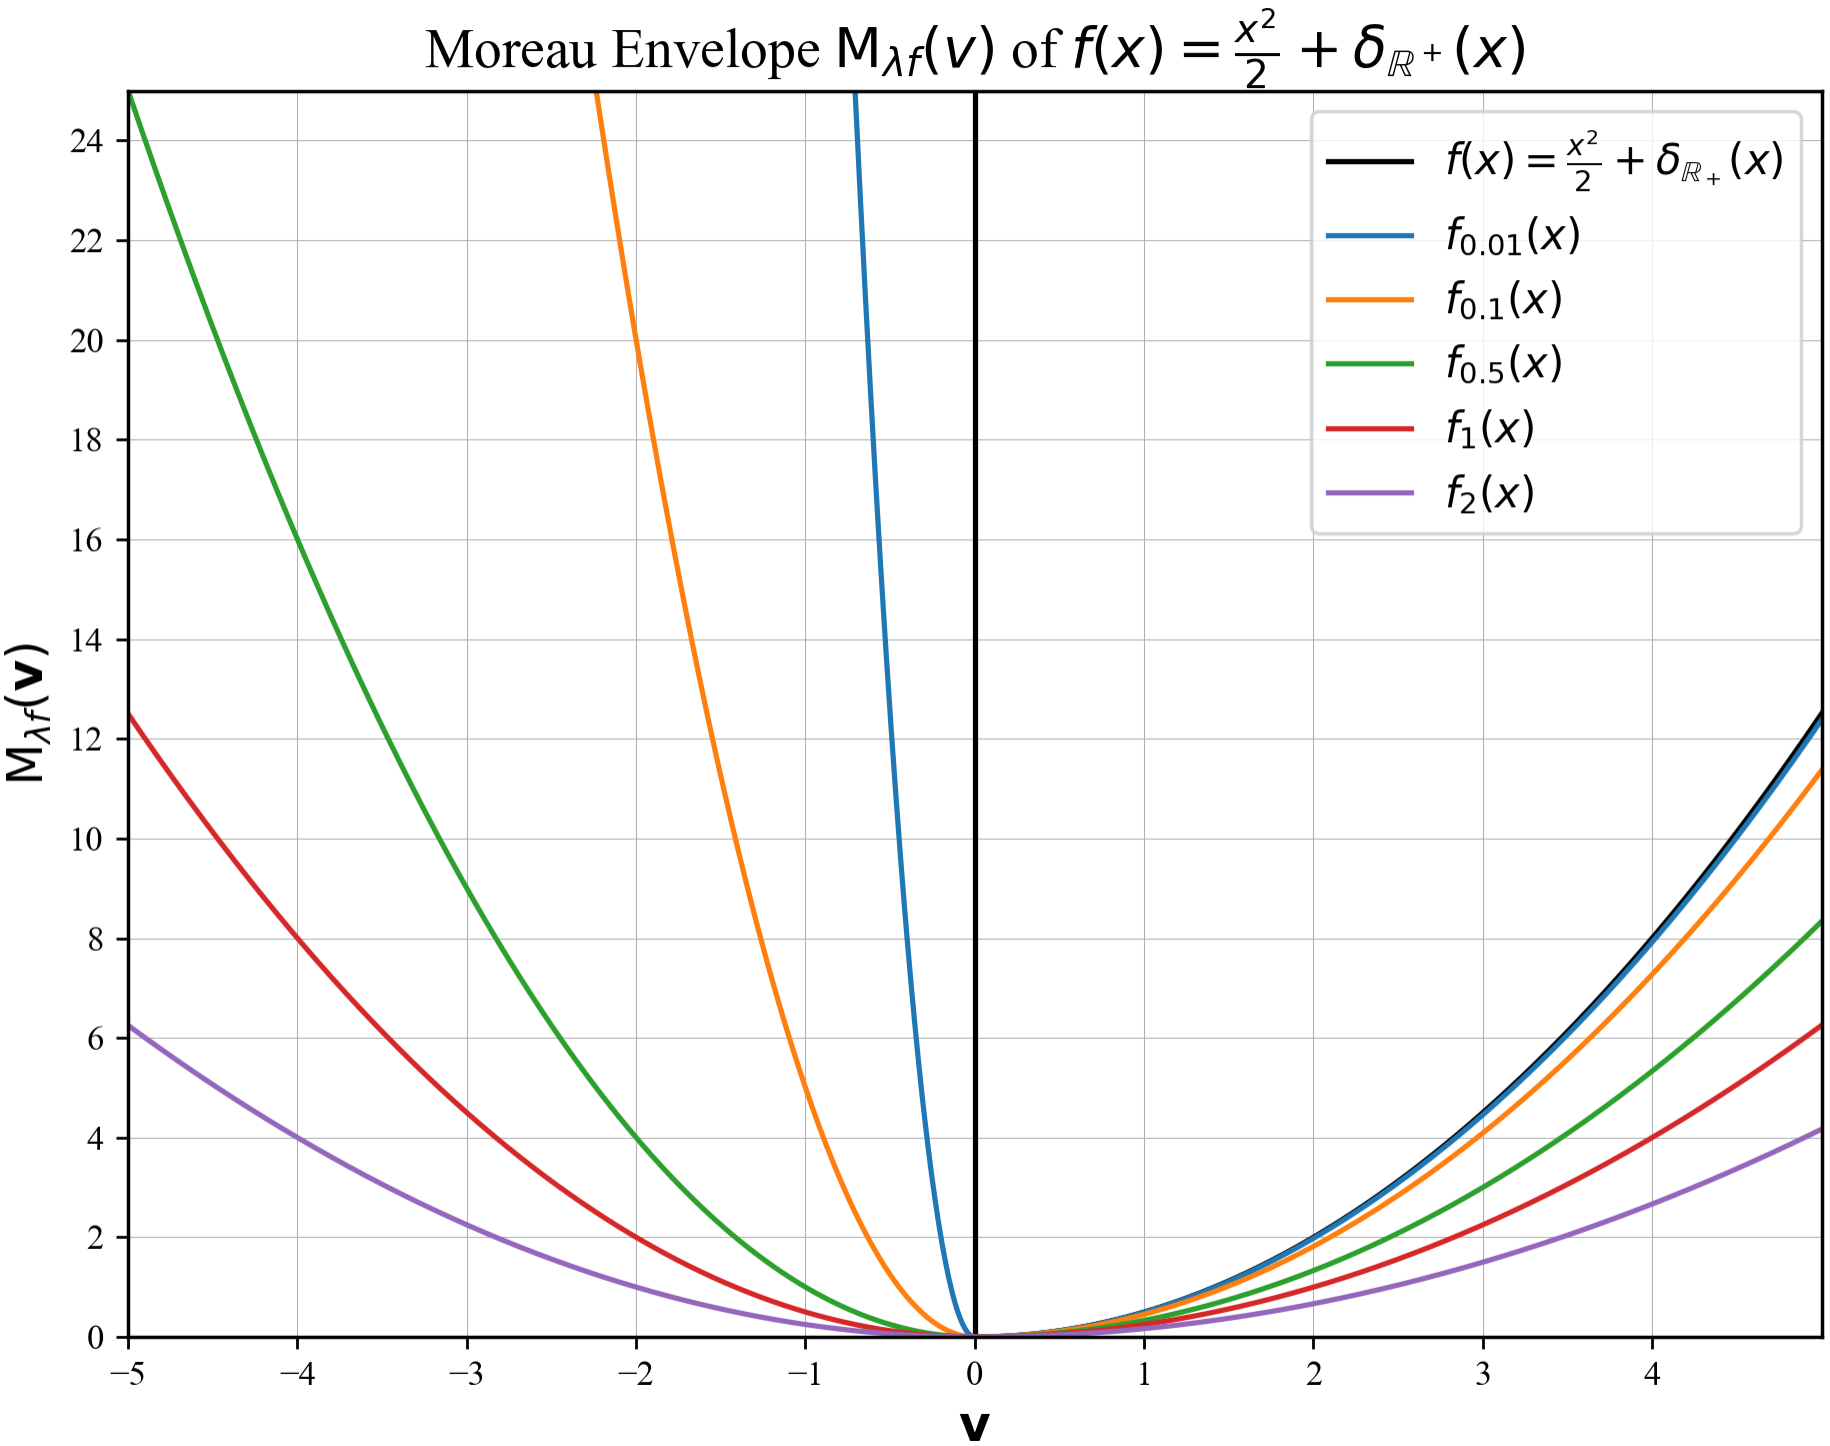
\includegraphics[width = 0.8\textwidth]{images/M_envelope.PNG}
  \caption{Moreau envelope $\mathrm{M}_{\lambda f}$ for $f = \frac{x^2}{2} + \delta_{\mathbb{R}_+}$ and different values of $\lambda$.} 
  \label{fig:moreau_envelope}
  \end{center}
\end{figure}

Figure \ref{fig:moreau_envelope} shows how $\mathrm{M}_{\lambda f}$, by adding a quadratic term to $f$ is basically a smoothed version of $f$, where the parameter $\lambda$ is a trade-off between fidelity to $f$ and smoothness. Furthermore $\mathrm{M}_{\lambda f}$ has several desirable qualities. Its domain is the whole set of real numbers $\mathbb{R}^n$, regardless of the domain of $f$. Moreover, it is continuously differentiable, even if $f$ is not, and the set of minimizers of $f$ and $\mathrm{M}_{\lambda f}$ is the same, which makes the minimization of $\mathrm{M}_{\lambda f}$ and $f$ equivalent problems. The advantage is that minimizing $\mathrm{M}_{\lambda f}$ is always a smooth problem, even though $\mathrm{M}_{\lambda f}$ can be difficult to evaluate. 

\subsubsection{Closed-form Solutions of Functions of Interest} \label{sect:prox_solutions}

\noindent\textbf{Indicator Function}

One particularly interesting case is the indicator function, for example the one given in  \eqref{eq:indicator_function}. Its proximal operator has a closed-form solution, and it is given by
\begin{equation}
\mathrm{prox}_{\lambda \delta_{\rm \mathbb{R}_+^N}}(\mathbf{v}) = \arg \min_\mathbf{x}(\delta_{\rm \mathbb{R}_+^N}+\frac{1}{2\lambda}||\mathbf{x} - \mathbf{v}||_2^2) = \arg \min_{\mathbf{x}\in \rm \mathbb{R}_+^N}\left(\frac{1}{2}||\mathbf{x} - \mathbf{v}||_2^2\right).
    \label{eq:prox_nonneg}
\end{equation}

As  \eqref{eq:prox_nonneg} demonstrates, the proximal operator of indicator functions is simply the projection from an input vector into the domain imposed by the function. For  \eqref{eq:indicator_function}, this domain is the set of real nonnegative numbers $\mathbb{R}_+^\mathrm{N}$. 

\noindent\textbf{Norms}

To evaluate the proximal operator of norms, the property known as \textit{Moreau decomposition} \cite{parikh_proximal_2014} is helpful. This property states that
\begin{equation}
\mathbf{v} = \mathrm{prox}_f(\mathbf{v}) + \mathrm{prox}_{f^*}(\mathbf{v}),
    \label{eq:moreau_dec}
\end{equation}
where $f^*$ is the conjugate function of $f$. This is very useful to evaluate proximal operators of norms, since their conjugate function is the indicator function $\mathcal{I}_{\mathcal{B}}$, where $\mathcal{B}$ is the unit ball of the norm. As aforementioned, the proximal operator of indicator functions has a closed form solution, and the problem of evaluating the proximal operator of norms reduces to evaluating the projection onto $\mathcal{B}$. Thus, \eqref{eq:moreau_dec} gives us a simple form of evaluating $\mathrm{prox}_{\lambda f}$. It follows that $\mathrm{prox}_f(\mathbf{v})$ parametrized with $\lambda$ is written as
\begin{equation}
\mathrm{prox}_{\lambda\ell_p}(\mathbf{v}) = \mathbf{v} - \lambda \Pi_{\mathcal{B}_p}(\frac{\mathbf{v}}{\lambda})
    \label{eq:norm_prox}
\end{equation}
And finding $\mathrm{prox}_{\lambda f}(\mathbf{v})$ can be done by finding $\Pi_{\mathcal{B}}(\frac{\mathbf{v}}{\lambda})$. 

Figure \ref{fig:prox_closed_form_sols} shows some element-wise plots of the closed-form solutions of functions of interest. Explicit derivations can be found in \cite{combettes_proximal_2007}. 
\begin{figure}[H]
  \begin{center}
  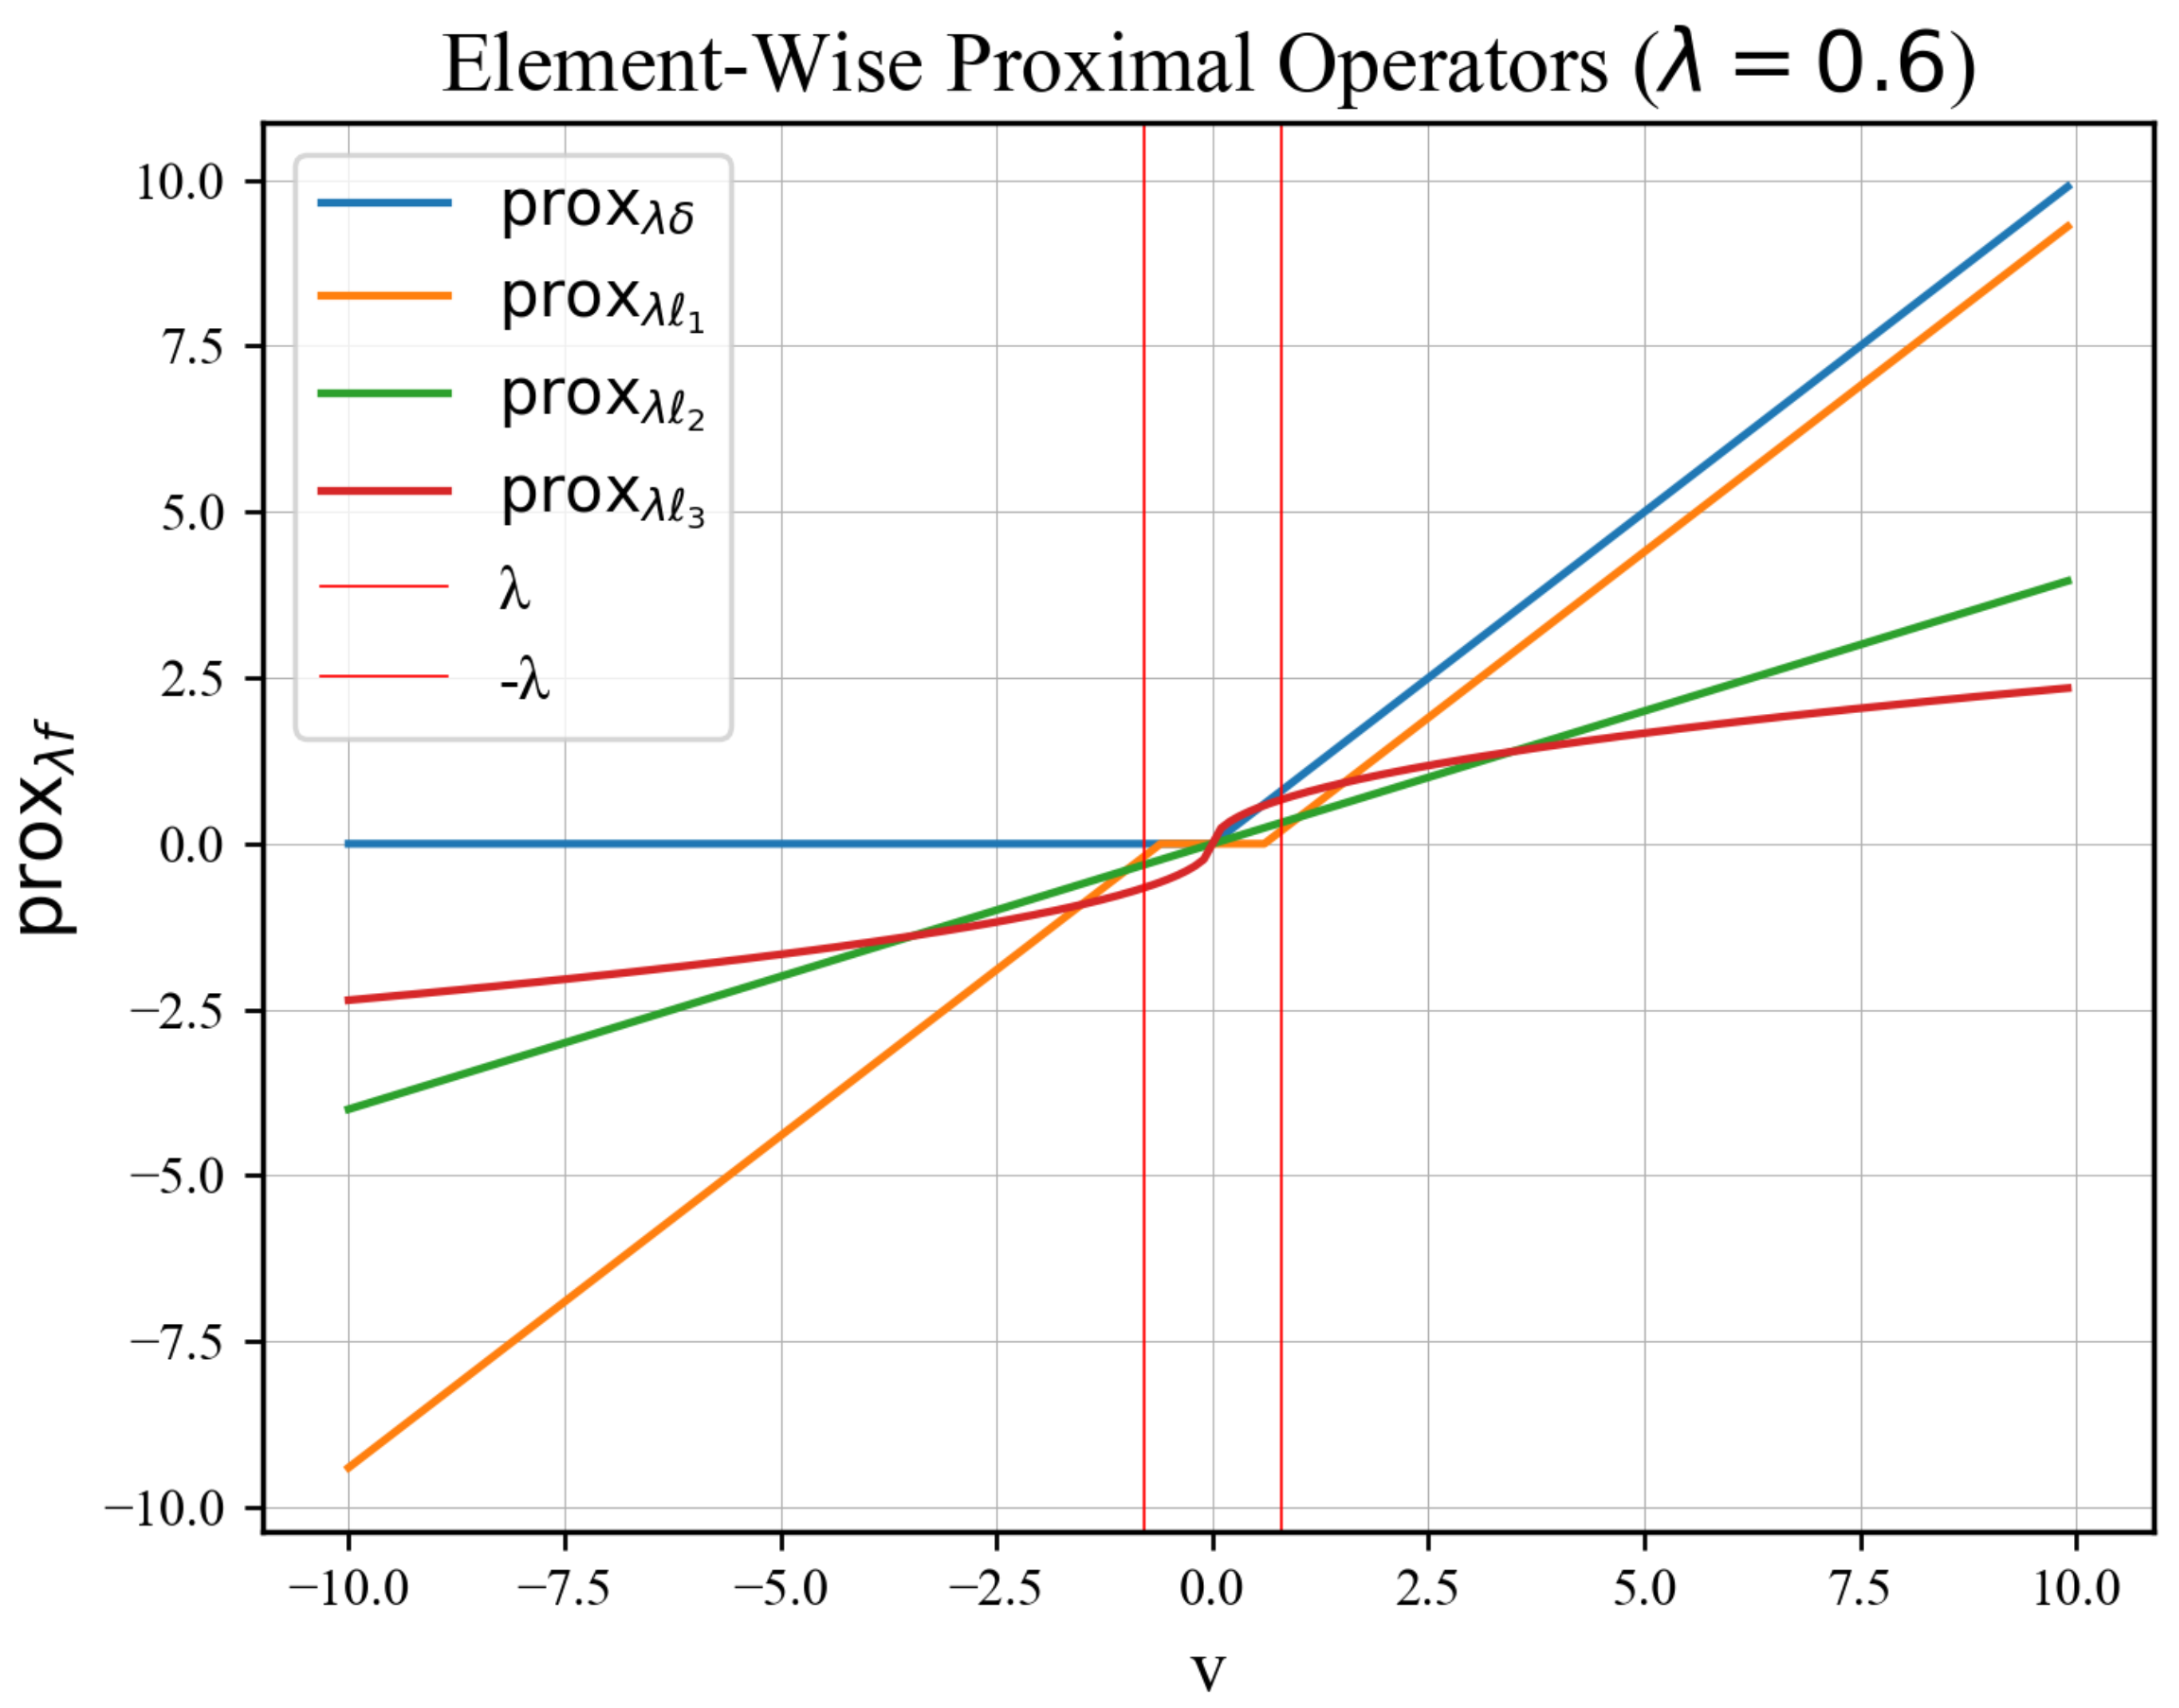
\includegraphics[width = 0.8\textwidth]{images/closed_form_sol_prox.PNG}
  \caption{Closed form solutions of element-wise proximal operators: $f = \delta_{\mathbb{R}_+^\mathrm{N}}$, $f = \ell_1$, $f = \ell_2$, and $f = \ell_3$. Note that $f = \ell_2$, and $f = \ell_3$ have been parametrized so that $\|\mathbf{v}\| = 1$.}
  \label{fig:prox_closed_form_sols}
  \end{center}
\end{figure}
In this simple functions, the effect of the proximal operator of $\ell_p$ norms and of $\delta_{\mathbb{R}_+^N}$ (defined in \eqref{eq:indicator_function}) is exemplified. For the nonnegativity constraints, where the proximal operator is the projection into $\mathbb{R}_+^\mathrm{N}$, we can see how nonnegative elements are left unchanged and negative elements are set to $0$. On the other hand, the proximal operator of the $\ell_1$ norm acts equivalently on all elements, bringing them closer to $0$ -without crossing it-, an operation called \textit{soft thresholding}. The proximal operator of the $\ell_2$ norm applies a linear transformation that depends on the value of the element $v_i$, parametrized by the norm of $\mathbf{v}$ (normalized to $1$ in Figure \ref{fig:prox_closed_form_sols}) and of course by $\lambda$. Norms of higher order have different behaviours for different values of $\mathbf{v}$, but we can see that in general they are element-wise operators.
 
% \subsubsection{Proximal Operators of Image Regularizers}

% To be included if there's time

\subsection{Proximal Optimization}

In this Section~I will describe some representative optimization algorithms that rely on the proximal operator. and are relevant in the context of image reconstruction.

\subsubsection{Example 1: Proximal Minimization}

The simplest algorithm is proximal minimization, where the update rule 
\begin{equation}
    \mathbf{x}^{k+1} := \mathrm{prox}_{\lambda f}(\mathbf{x}^k)
    \label{eq:prox_minimization}
\end{equation}
is simply applying the proximal operator on the current value.
In  \eqref{eq:prox_minimization}, $f$ is still a closed convex scalar function, $\mathbf{x}$ is the optimization variable, and $k$ is the iteration counter. One step of the proximal optimization algorithm is shown in figure \ref{fig:proximal_minimization}. 

\begin{figure}[H]
  \begin{center}
  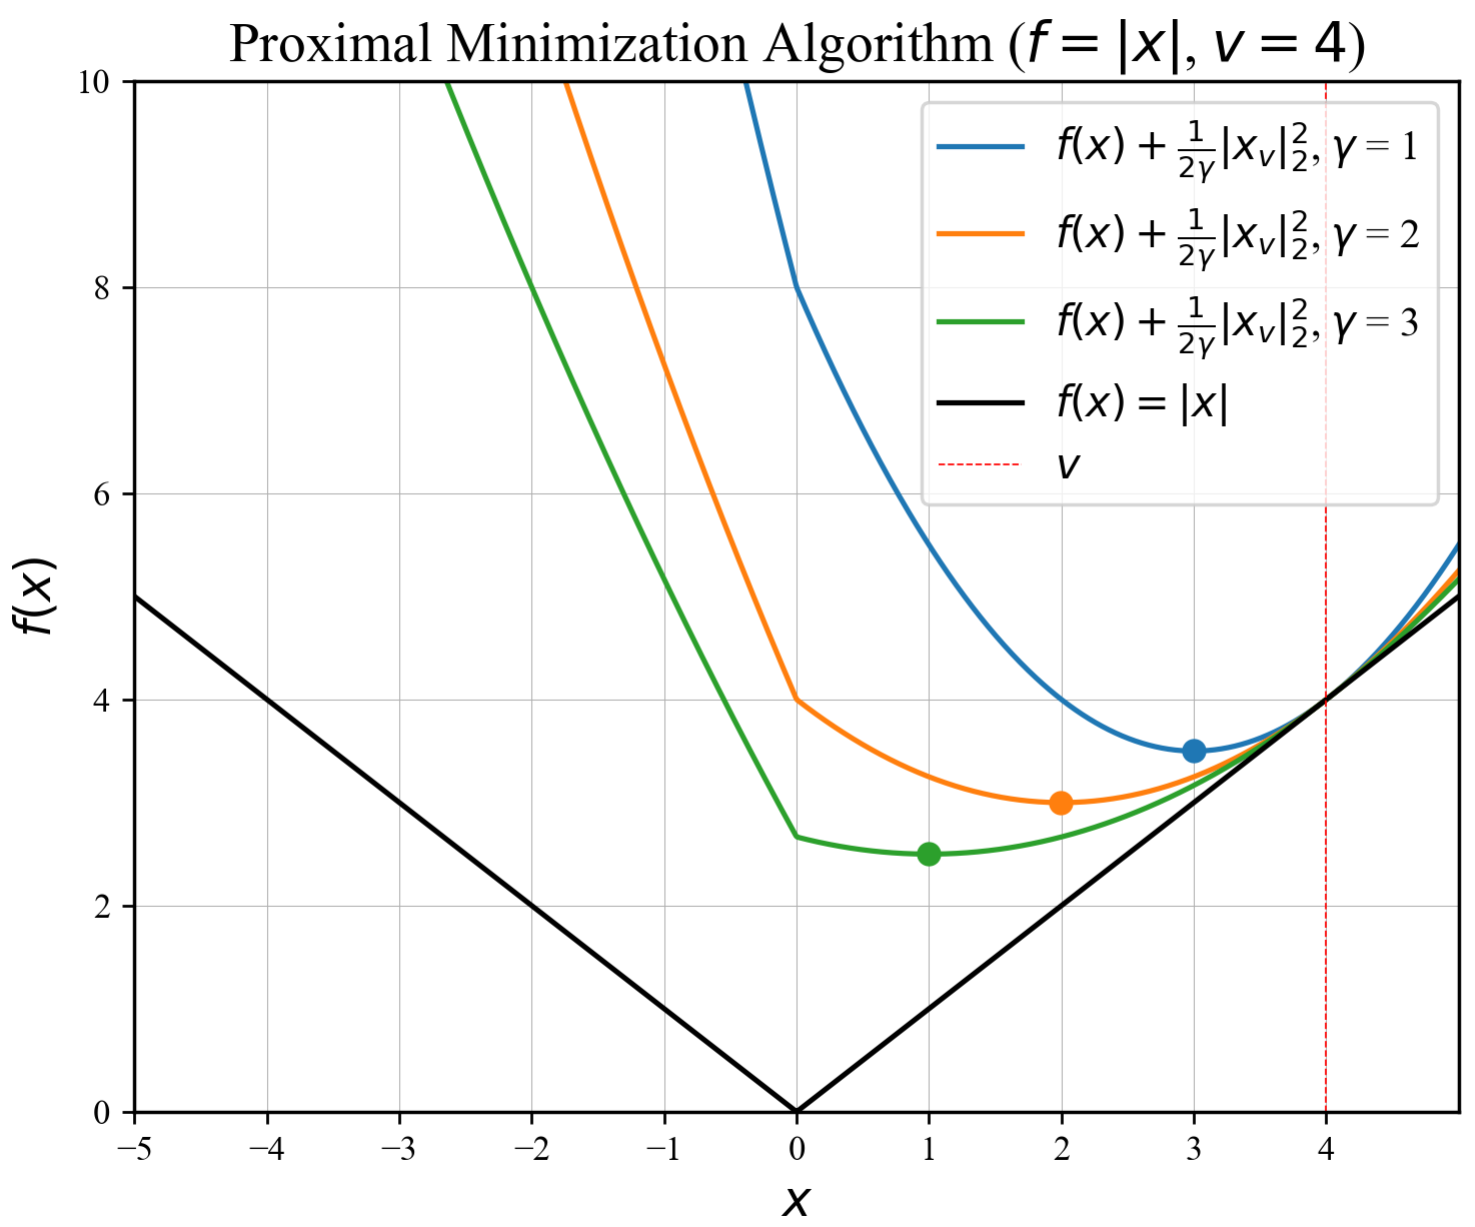
\includegraphics[scale = 0.7]{images/Proximal_minimization.PNG}
  \caption{Proximal minimization algorithm \eqref{eq:prox_minimization}. The image shows one step of the proximal minimization algorithm applied to the simple function $f(x) = |x|$ (in black). Three different values of $\lambda \in \{1, 2, 3\}$ are shown. The whole objective function is shown, and its minimum -the result of the proximal operator- is indicated in the plot.}
  \label{fig:proximal_minimization}
  \end{center}
\end{figure}

In figure \ref{fig:proximal_minimization}, the function $f(x) = |x|$ is minimized via the proximal minimization algorithm, arbitrarily choosing $v = 4$ as starting point. The objective function of the proximal operator is plotted for $\lambda \in \{1, 2, 3\}$. Note how, since $f(x)$ is the $\ell_1$ norm of a scalar, figure \ref{fig:proximal_minimization} is in complete agreement with figure \ref{fig:prox_closed_form_sols}, where it is shown the the element wise operation of $\mathrm{prox}_{\lambda \ell_1}$ is soft thresholding, with $\lambda$ as a threshold.

\subsubsection{Example 2: Proximal Gradient Method}
An algorithm that has found further applications is the \textit{proximal gradient method}. It acts on a convex objective function $f+g$, where $f: \mathbb{R}^\mathrm{N} \rightarrow \mathbb{R} $ is smooth and differentiable, but $g: \mathbb{R}^\mathrm{N} \rightarrow \mathbb{R} \bigcup \{+\infty \}$ is not. Note that since $g$ includes $\infty$ it can be the indicator function in  \eqref{eq:imaging_problem}. 

The proximal gradient method update rule is given by:
\begin{equation}
    \mathbf{x}^{k+1} := \mathrm{prox}_{\lambda g}(\mathbf{x}^k - \lambda^k \nabla f(\mathbf{x}^k)),
    \label{eq:prox_gradient_descnet}
\end{equation}
where the minimization objective is split into two, $f$ and $g$. Then, an iteration over the whole objective includes a gradient step in $f$ -note that $f$ is both smooth and differentiable- , and a a proximal minimization step in $g$. If $g$ is an indicator function, then as  \eqref{eq:prox_nonneg} shows, the minimization step over $g$ is the projection on the valid set, and the proximal gradient method becomes equivalent to projected gradient descent. %This scenario is illustrated in Figure \ref{fig:projected_grad_descent}  .

% \begin{figure}[H]
%   \begin{center}
%   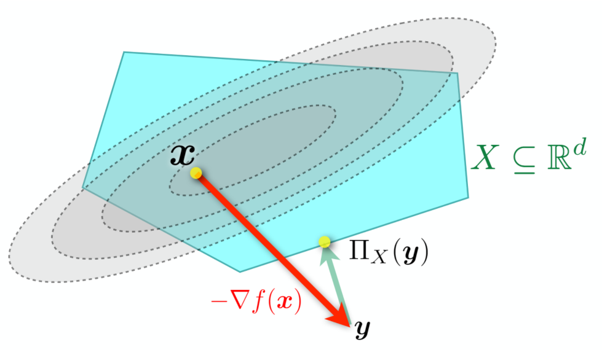
\includegraphics[width = 0.8\textwidth]{images/Projected_grad_descent.png}
%   \caption{proximal gradient method algorithm When $g$ in  \eqref{eq:prox_gradient_descnet} is an indicator function, it reduces to projected gradient mescent. Figure reuused from \href{https://github.com/epfml/OptML_course/blob/master/slides/lecture03.pdf}{CS-439 course notes}.}
%   \label{fig:projected_grad_descent}
%   \end{center}
% \end{figure}

% \begin{equation}
%     \mathrm{where}\;\;\;\; \mathbf{v} = \mathbf{x} - \lambda \nabla f(\mathbf{x})
%     \label{eq:prox_gradient_descnet}
% \end{equation}


% $\mathbf{z}_n,\; \mathbf{u}\;\in \mathbb{R}^N$

% $\mathrm{prox}_{\lambda g}, \mathrm{prox}_{\lambda f} \rightarrow$ optimization problems

\subsubsection{Example 3: ADMM} \label{sect:admm}

The alternating direction method of multipliers (ADMM) \cite{boyd_distributed_2011} is a method for minimizing objective functions of the form.
\begin{equation}
    % F_0(\mathbf{x}) + \Sigma_{n=1}^{N}F_n(\mathbf{H}_n\mathbf{x}),
    \sum_{n=1}^{N}F_n(\mathbf{H}_n\mathbf{x}),
    \label{eq:ADMM_obj}
\end{equation}
where, as before, $\mathbf{x} \in \mathbb{R}^N$, and each term of the summation has a linear operator $\mathbf{H}_n: \mathbb{R}^N \rightarrow \mathbb{R}^{Q_n}$ acting on $\mathbf{x}$ and a scalar function $F_n: \mathbb{R}^{Q_n} \rightarrow \mathbb{R}$ that has $\mathbf{H}_n\mathbf{x}$ as input. This form clearly represents \eqref{eq:imaging_problem}, since it is formed out of three separable functions, each with its own transforms and functions. For $n = 1$, the transform $\mathbf{H}_1 = \mathbf{H}$ is the forward model and $F_1 = \mathcal{D}$ is the data fidelity metric. For $n=2$, shown in \eqref{eq:regularizer}, $\mathbf{H}_2 = \mathbf{L}$ and $F_2 = \operatorname{R}$, and for $n=3$, the nonnegativity constraint, $\mathbf{H}_3 = \mathbf{I}$ is the identity operator and $F_n = \delta_{\mathbb{R}^N_+}$. Moreover, $F_n$ for all $n$ needs to be convex, but need not be neither differentiable nor smooth. Therefore, from the examples we have seen, ADMM has the broadest applicability and is one of the most relevant algorithms for image reconstruction tasks. 

The principle of ADMM is to find a saddle point of the scaled augmented Lagrangian formulation of \eqref{eq:ADMM_obj}, given by
\begin{equation}
    \mathcal{L}_{\rho}(\mathrm{\mathbf{x}},\mathbf{y}_1, …, \mathbf{y}_n,\mathbf{w}_1, …, \mathbf{w}_n) = \sum_{n=1}^N \frac12\rho_n\left\| \mathrm{\mathbf{H}_n\mathbf{x} - \mathbf{y}_n + \frac{\mathbf{w}_n}{\rho_n}}\right\|^2 + F_n(\mathrm{\mathbf{y}_n}),
    \label{eq:scaled_lag}
\end{equation}
through the update rules
\begin{equation}
    \begin{split}
    \mathbf{x}^{k+1} &:= \arg\min_\mathbf{x}\mathcal{L}_{\rho}(\mathbf{x},\mathbf{y}_1^k, …, \mathbf{y}_n^k,\mathbf{w}_1^k…\mathbf{w}_n^k)\\
    \mathbf{y}_1^{k+1} &:= \arg\min_{\mathbf{y}_1}\mathcal{L}_{\rho}(\mathbf{x}^{k+1},\mathbf{y}_1, …, \mathbf{y}_n,\mathbf{w}_1^k…\mathbf{w}_n^k)\\
    &\vdots\\
    \mathbf{y}_n^{k+1} &:= \arg\min_{\mathbf{y}_n}\mathcal{L}_{\rho}(\mathbf{x}^{k+1},\mathbf{y}_1, …, \mathbf{y}_n,\mathbf{w}_1^k…\mathbf{w}_n^k)\\
    \mathbf{w}_1^{k+1} &:= \mathbf{w}_1^k + \rho(\mathbf{x}^{k+1}-\mathbf{y}^{k+1}_1)\\
    &\vdots\\
    \mathbf{w}_n^{k+1} &:= \mathbf{w}_n^k + \rho(\mathbf{x}^{k+1}-\mathbf{y}^{k+1}_n).\\
    \end{split}
    \label{eq:admm_update}
\end{equation}
Since $\mathcal{L}_\rho$ is separable accross $n$, an update step only acts on the terms of the corresponding summation. As such, the explicit update step of $\mathbf{y}_n$ is
\begin{equation}
    \mathbf{y}_n^{k+1} := \arg\min_{\mathbf{y}_n}\left(F_n(\mathbf{y}_n) + \frac{\rho}{2} \left\|\mathbf{H}_n\mathbf{x} - \mathbf{y}_n - \frac{1}{\rho}\mathbf{w}^k_n\right\|^2 \right) = \mathrm{prox}_{ F_n\lambda}(\mathbf{x}^{k+1} - \mathbf{w}^k_n), 
    \label{eq:admm_explicit_update}
\end{equation}
Where we have made $\lambda = 1/\rho$. 

Therefore, ADMM is a common choice when the proximal operator of $f = F_n$,  $\mathrm{prox}_{ F_n\lambda}(\mathbf{v})$ is known, but the proximal operator of $f = F_n +F_{n+1}$, $\mathrm{prox}_{(F_n+F_{n+1})\lambda}(\mathbf{v})$, is not known or it is hard to evaluate, as it is the case for combinations norms with nonnegativity constraints.
% \begin{equation}
%     \begin{split}
%     \mathbf{x}^{k+1} &:= \mathrm{prox}_{\lambda f}(\mathbf{z}^k - \mathbf{u}^k)\\
%     \mathbf{z}_n^{k+1} &:= \mathrm{prox}_{\lambda g_n}(\mathbf{x}^{k+1} - \mathbf{u}^k)\\
%     \mathbf{u}^{k+1} &:= \mathbf{u}^{k+1} + \operatorname{A}\mathbf{x}^{k+1} + \operatorname{B}\mathbf{z}^{k+1}\\
%     \end{split}
%     \label{eq:prox_gradient_descnet}
% \end{equation}

% \subsubsection{Known Proximal Operators}

% Projection
% \begin{equation}
%     \begin{split}
%     \Pi_\matcal{C}(\mathbf{v}) = \arg \min_{\mathbf{x}\in \mathcal{C}}\|\mathbf{x} - \mathbf{v}\|_2
%     \end{split}
%     \label{eq:prox_gradient_descnet}
% \end{equation}

% $\mathrm{prox}_{\lambda \|\cdot \|_2}(\mathbf{v}) = \left(1 - \frac{\lambda}{\min \left( \|\mathbf{v}\|_2, \lambda \right)}\right) \mathbf{v}$

% $\mathrm{sgn}(\mathbf{x})\mathrm{max}(|\mathbf{x}| - \lambda, 0)$

% $\Pi_\matcal{C}(\mathbf{v}) = \arg \min_{\mathbf{x}\in \mathcal{C}}\|\mathbf{x} - \mathbf{v}\|_2$
\subsection{Scope of the Project} \label{sect:1.scope}

One of the drawbacks of solving an inverse imaging problem through  \eqref{eq:imaging_problem} is the splitting required to use ADMM. This splitting results in the need to optimize two additional variables of the same size of the original per extra function. Consequently, this project aims to mitigate this issue by investigating the combination of the proximal operator of common image regularizers with nonnegativity constraints. 

In other words, we will study the $\mathrm{prox}_{\lambda f}(x)$ for
\begin{equation}
    f(\mathbf{x}) = \mathcal{R}(\mathbf{x}) + \delta_{\rm \mathbb{R}_+^N}(\mathbf{x}),
    \label{eq:scope_objective}
\end{equation}
and by combination it is meant taking first the proximal of one of the two functions in $f$, then the proximal of the other function, and then check whether they are equal to $\mathrm{prox}_f$. The goal is to find regularizers for which one of the following two conditions
\begin{equation}
    \mathrm{prox}_{\mathcal{R} + \delta_{\rm \mathbb{R}_+^N}}(\mathbf{x}) =  \mathrm{prox}_{\delta_{\rm \mathbb{R}_+^N}}(\mathrm{prox}_{\mathcal{R}}(\mathbf{x}))\mbox{, or}
    \label{eq:prox_nonneg(prox_r)}
\end{equation}
\begin{equation}
    \mathrm{prox}_{\mathbb{R} + \delta_{\rm \mathbb{R}_+^N}}(\mathbf{x}) = \mathrm{prox}_{\mathcal{R}}(\mathrm{prox}_{\delta_{\rm \mathbb{R}_+^N}}(\mathbf{x}))
    \label{eq:prox_r(prox_nonneg)}
\end{equation}
are met. This has been exploited before in \cite{del_aguila_pla_cell_2018-1, del_aguila_pla_cell_2018} and the conditions for it to happen is a topic of active research in convex analysis \cite{Adly2019}.  

If, for a given regularizer, any of the two equations \ref{eq:prox_nonneg(prox_r)} and \ref{eq:prox_r(prox_nonneg)} hold, it is possible to reconstruct an image using the right-hand side of the valid equation. This means that there is no need to treat $\mathcal{R}$ and $\delta$ separately, which has the advantage of not having to store the extra variables generated during ADMM splitting. Therefore, this study has the potential of significantly reducing the computational and memory load of solving imaging problems.



% % \newpage
\section{Methods} \label{sect:2_methods}

\subsection{Computational Environment} \label{sect:2environment}
All the experiments were carried out in Jupyter Notebooks, with Python version 3.7.9, using standard libraries like NumPy, SciPy and Matplotlib. To obtain most proximal operators, I used CVXPy, a Python modelling library to solve convex optimization problems, using the solver MOSEK. This adapts well to image regularizers, since, as it was explained in Section \ref{sect:2regularizers}, they are convex functions.  

Specific library versions are found in the \href{https://github.com/Alejandro-1996/ProximalOperatorsProject/requirements.txt}{requirements} file of the \href{https://github.com/Alejandro-1996/ProximalOperatorsProject}{project's Github repository}. Furthermore, all the Jupyter Notebooks are found in the same repository. 

\subsection {Evaluating Combination of $\mathcal{R}$ with $\delta_{R_+^N}$}  \label{sect:2evaluating}

To validate each of \eqref{eq:prox_nonneg(prox_r)} and \eqref{eq:prox_r(prox_nonneg)}, I first created a random array ($1$-dimensional or $2$-dimensional as required by the regularizer), and then used CVXPy to calculate the right-hand and the left-hand sides of both equations. Then, I created an error array, to calculate and store the maximum and average errors. The process was repeated $100$ times on different arrays (of the same size and sampled from the same distribution) and the average and maximum errors were taken over the results of the $100$ arrays.

% \begin{itemize}
%     \item Create random array ($1D$ or $2D$, depending on the regularizer to test).
%     \item Apply left hand side of equations.
%     \item Apply right hand side (for both equations).
%     \item Check for equality.
% \end{itemize}

% \usetikzlibrary{shapes.geometric, arrows}
% \tikzstyle{startstop} = [rectangle, rounded corners, minimum width=3cm, minimum height=1cm,text centered, draw=black, fill=red!30]
% \tikzstyle{io} = [trapezium, trapezium left angle=70, trapezium right angle=110, minimum width=3cm, minimum height=1cm, text centered, draw=black, fill=blue!30]
% \tikzstyle{process} = [rectangle, minimum width=3cm, minimum height=1cm, text centered, text width=3cm, draw=black, fill=orange!30]
% \tikzstyle{decision} = [diamond, minimum width=3cm, minimum height=1cm, text centered, draw=black, fill=green!30]
% \tikzstyle{arrow} = [thick,->,>=stealth]

% \begin{tikzpicture}[node distance=2cm]

% \node (start) [startstop] {Start};
% \node (in1) [io, below of=start] {Create Random Array};
% \node (pro1) [process, below of=in1] {Evaluate rhs and lhs of  \eqref{eq:prox_nonneg(prox_r)} and \eqref{eq:prox_nonneg(prox_r)}};
% \node (pro2) [process, below of=pro1] {Keep track of $\nabla = rhs - lhs$ for both \eqref{eq:prox_nonneg(prox_r)} and \eqref{eq:prox_nonneg(prox_r)} };
% \node (pro3) [process, below of=pro2] {Calculate average errors (over 100 runs)}; 
% \node (dec1) [decision, below of=pro3, yshift=-0.5cm] {Hola};{Decide whether \eqref{eq:prox_nonneg(prox_r)} and \eqref{eq:prox_nonneg(prox_r)} are true};
% \node (out1) [io, below of=dec1] {Print};
% \node (stop) [startstop, below of=out1] {Stop};

% \draw [arrow] (start) -- (in1);
% \draw [arrow] (in1) -- (pro1);
% \draw [arrow] (pro1) -- (pro2);
% \draw [arrow] (pro2) -- (pro3);
% \draw [arrow] (pro2) |- node[anchor=east] {Repeat $100$ times} (in1);
% % \draw [arrow] (pro3) -- node[anchor=south] {no} (pro2);
% \draw [arrow] (pro3) -- (dec1);
% \draw [arrow] (dec1) -- (out1);
% % \draw [arrow] (pro2a) -- (out1);
% \draw [arrow] (out1) -- (stop);


% \end{tikzpicture}

% \begin{itemize}
%     \item Create random array ($1D$ or $2D$, depending on the regularizer to test).
%     \item Apply left hand side of equations.
%     \item Apply right hand side (for both equations).
%     \item Check for equality.
% \end{itemize}

To generate the input random arrays, I used Gaussian (with $\mu = 0$ and $\sigma \in [1, 255$])) and uniform distributions in several ranges ($[0,1], [0,100], [0,255]$). Since CVXPy solves optimization problems numerically, there is never a complete equality of both arrays, and an arbitrary decision has to be taken on whether \eqref{eq:prox_nonneg(prox_r)} and \eqref{eq:prox_r(prox_nonneg)} are valid or not. As a general trend, the more complex the regularizer (i.e, the more CVXPy functions are used) the lower accuracy, and the larger the arrays the bigger the accuracy. This of course results in computational constraints on the size of the arrays, a constraint that is more relevant for complex regularizers. Consequently the decision on whether two expressions are evaluated to be equal will be explained in a case by case basis in Section \ref{sect:3}.

\subsection{Experiments}

For some complex regularizers of interest, and to compare the results and behaviour on real images, I performed some experiments. These were done on much larger images than the ones use during the experimental procedure, in which the true behaviour of the regularizer is clearly visible. The downside of this experiments is that they are too computationally demanding to perform many of them. 

In particular, I did 2 experiments, one for nonisotropic $\operatorname{TV}$ regularization and one for Hessian-Schatten norm regularization. In both cases, I took a standard test image, normalized it to the range $[0, 1]$, and added white noise to it. Then, I used it as the input of the left-hand side and right hand side of \eqref{eq:prox_nonneg(prox_r)} and \eqref{eq:prox_r(prox_nonneg)}. For an analysis on the results, I compared them visually, calculated the numerical differences and calculated the $\mathrm{SNR}$ to the original.







% \newpage
\section{Results} \label{sect:3}

In this section I will present the results of the evaluation of \eqref{eq:prox_nonneg(prox_r)} and \eqref{eq:prox_r(prox_nonneg)}, for \textit{simple} regularizers (e.g. norms acting on the raw arrays) to more complex, state-of-the-art image regularizers. In these cases, I will also present some experiments on standard test images. A summary of the results is presented in Table \ref{tab:exp_results}.

\begin{center}
    \begin{table}[H]
    \begin{tabular}{||c|c|c|c|c|c||}
        \hline
        %%%%%%%%%%%%%%%%%%%%%% HEADING %%%%%%%%%%%55
        Dimension & $\mathbf{L}$ & $\operatorname{R}$ & $\mathrm{prox}_{\delta}(\mathrm{prox}_{\mathcal{R}}(\mathbf{v}))$ & $\mathrm{prox}_{\mathcal{R}}(\mathrm{prox}_{\delta}(\mathbf{v}))$ & Parameters \cr 
        \hline \hline
        
        %%%%%%%%%%%%%%%%%%%%55 PReviousely Known casesw %%%%%%%
        1, 2 & $\operatorname{I}$ & $\|\cdot\|_1$ &  \checkmark ($10^{-5}$)& \checkmark ($10^{-7}$) & $\mathcal{N}(0, 1)$, $x\in \mathbb{R}^{100}$\\ 
        1, 2 & $\operatorname{I}$ &  $\|\cdot\|_2$ & $\times$($10^{-3}$)& \checkmark ($10^{-6}$)&$\mathcal{N}(0, 1)$, $x\in \mathbb{R}^{100}$\cr \hline
        
        %%%%%%%%%%%% Identity 
        1, 2 & $\operatorname{I}$ &  $\|\cdot\|_p$ & $\times$($10^{-3}$) & \checkmark ($10^{-7}$) & $\mathcal{N}(0, 1)$, $x\in \mathbb{R}^{100}$\\
        1, 2 & $\operatorname{I}$ & $\|\cdot\|_p^p$ & \checkmark ($10^{-6}$) & \checkmark ($10^{-6}$) & $\mathcal{N}(0, 1)$, $x\in \mathbb{R}^{100}$\\
        2 & $\operatorname{I}$ & $\|\cdot\|_{S_1}$ &  $\times$ ($10^{-2}$) & $?$ ($10^{-3}$) & $\mathcal{N}(0, 100)$, $x\in \mathbb{R}^{2 \times 2}$ \\
        2 & $\operatorname{I}$ & $\|\cdot\|_{S_2}$ &  $\times$ ($10^{-2}$) & $?$ ($10^{-3}$) & $\mathcal{N}(0, 100)$, $x\in \mathbb{R}^{2 \times 2}$ \\
        2 & $\operatorname{I}$ & $\|\cdot\|_{S_3}$ &  $\times$ ($10^{-2}$) & $?$ ($10^{-3}$) & $\mathcal{N}(0, 100)$, $x\in \mathbb{R}^{2 \times 2}$\cr\hline
        
        %%%%%%%%%%%% Total Viariation 
        1 & $\nabla_1$ & $\|\cdot\|_1$ & \checkmark ($10^{-6}$)& $\times$ ($10^{-1}$) & $\mathcal{N}(0, 1)$, $x\in \mathbb{R}^{50}$ \\
        1 & $\nabla_1$ & $\|\cdot\|_p$ & $\times$ ($10^{-2}$) & $\times$ ($10^{-2}$) & $\mathcal{N}(0, 1)$, $x\in \mathbb{R}^{50}$\\
        1 & $\nabla_1$ & $\|\cdot\|_p^p$ & $\times$ ($10^{-2}$) & $\times$ ($10^{-2}$) & $\mathcal{N}(0, 1)$, $x\in \mathbb{R}^{50}$ \\
        2 & $\nabla_2$ & $\|\cdot\|_{1, 1}$ &  \checkmark ($10^{-7}$)& $\times$ ($10^{-1}$) & $\mathcal{N}(0, 1)$, $x\in \mathbb{R}^{40\times 40}$\\
        2 & $\nabla_2$ & $\|\cdot\|_{p, q}$ & $\times$ ($10^{-2}$)& $\times$ ($10^{-1}$) & $\mathcal{N}(0, 1)$, $x\in \mathbb{R}^{40\times 40}$\\
        2 & $\nabla_2$ & $\|\cdot\|_{p, q}^{p, q}$ & $\times$ ($10^{-1}$)& $\times$ ($10^{-1}$) & $\mathcal{N}(0, 1)$, $x\in \mathbb{R}^{40\times 40}$\cr \hline
        
        %%%%%%%%%%%%%%%%%%%%%%%%%% Group Sparsity
        1, 2 &  $\operatorname{I}$ & $\|\cdot\|_{1, 1}$  & \checkmark ($10^{-7}$) & \checkmark ($10^{-7}$) & $\mathcal{N}(0, 1)$, $x\in \mathbb{R}^{40 \times 40}$\\
        1, 2 &  $\operatorname{I}$ & $\|\cdot\|_{p, q}$  & $\times$ ($10^{-2}$)& \checkmark ($10^{-6}$) & $\mathcal{N}(0, 1)$, $x\in \mathbb{R}^{40 \times 40}$\\
        1, 2 &  $\operatorname{I}$ & $\|\cdot\|_{p, q}^{p, q}$  & $\times$ ($10^{-4}$)& \checkmark ($10^{-7}$) & $\mathcal{N}(0, 1)$, $x\in \mathbb{R}^{40 \times 40}$\\
        1, 2 &  $\operatorname{I}$ & $\|\cdot\|_{1, q}$  &  \checkmark ($10^{-7}$)& \checkmark ($10^{-7}$) & $\mathcal{N}(0, 1)$, $x\in \mathbb{R}^{40 \times 40}$ \\
        1, 2 &  $\operatorname{I}$ & $\|\cdot\|_{p, 1}^{p, q}$  &  \checkmark ($10^{-7}$) & \checkmark ($10^{-7}$) & $\mathcal{N}(0, 1)$, $x\in \mathbb{R}^{40 \times 40}$ 
        \cr \hline
        
        %%%%%%%%%%%%%%%%%%%%%%%%%% Hessian Schatten + DCT
        % 1 & $\operatorname{DCT}$ &  $\ell_1$ & $\times$& $\times$ & \cr\hline
        % 2 & $\operatorname{HS}$ & $\ell_*$ & Seems & $\times$ &\\
        2 & $\operatorname{HS}$ & $\|\cdot\|_{S_1, p}$ &  $\times$ ($10^{-1}$) & $\times$ ($10^{-1}$) & $\mathcal{N}(0, 10)$, $x\in \mathbb{R}^{15 \times 15}$\\ 
        2 & $\operatorname{HS}$ & $\|\cdot\|_{S_2, p}$ &  $\times$ ($10^{-1}$) & $\times$ ($10^{-1}$) & $\mathcal{N}(0, 10)$, $x\in \mathbb{R}^{15 \times 15}$\\
        2 & $\operatorname{HS}$ & $\|\cdot\|_{S_{\infty}, p}$ &  $\times$ ($10^{-1}$) & $\times$ ($10^{-1}$) & $\mathcal{N}(0, 10)$, $x\in \mathbb{R}^{15 \times 15}$ \cr\hline
    \end{tabular}
    \caption{\label{tab:exp_results} Experimental Results. The first three columns describe the regularizer $\mathcal{R}$, while the fourth and fifth columns present the results obtained with the average absolute error. The last column shows the parameters used to obtain the presented results. In all cases, $100$ different arrays were sampled and tested, and the average absolute error is presented over the hundred samples. The first two rows show results that were previously known, and are therefore useful to test the setup of the project. The rest of the lines separate the table by transform applied to the original signal/image. The second block corresponds to simple norms, the third block to $\operatorname{TV}$ regularizers, the fourth one to Group Sparsity regularizers and the fifth block to Hessian-Schatten norm regularizers.}
    \end{table}
\end{center}

As explained in section \ref{sect:2environment}, I used CVXPy to evaluate all image regularizers, constructing them in terms of combinations of simple convex functions. In particular, for the derivatives needed to calculate $\operatorname{TV}$ and the Hessian-Schatten norm, I used only the valid region of the resulting array, to avoid boundary artifacts. 

\noindent\textbf{$\ell_1$, $\ell_2$ norm} 

The $\ell_1$ and $\ell_2$ norms were studied with the purpose of validating the experimental setup, as these results are already known in the literate \cite{del_aguila_pla_cell_2018}. Moreover, as presented in section \ref{sect:prox_solutions}, and depicted in figure \ref{fig:prox_closed_form_sols}, there is a closed-form solution. However, I still used the experimental setup as a validation of the methodology. 

As shown in table \ref{tab:exp_results}, the results agree with the literature. In the case of the $\ell_1$ norm, both \eqref{eq:prox_nonneg(prox_r)} and \eqref{eq:prox_r(prox_nonneg)} are valid for $\mathcal{R} = \ell_1$, with average absolute errors in the order of $10^{-5}$ for  \eqref{eq:prox_r(prox_nonneg)} and of $10^{-7}$ for  \eqref{eq:prox_nonneg(prox_r)}. In the case of $\mathcal{R} = \ell_2$, I also recovered the results presented in \cite{del_aguila_pla_cell_2018}. I found that  \eqref{eq:prox_r(prox_nonneg)} is valid with average absolute errors in the order of $10^{-6}$, while  \eqref{eq:prox_nonneg(prox_r)} does not hold true, with average absolute errors in the order of $10^{-3}$. 

This error rates, applied on simple regularizers and with $1$-dimensional and $2$-dimensional, reasonably big arrays, provide guidelines on what I will consider to validate or not equations \eqref{eq:prox_nonneg(prox_r)} and \eqref{eq:prox_r(prox_nonneg)}.

\noindent\textbf{$\ell_p$ and $\ell_p^p$ norms} 

After validating the experimental methodology, I made an investigation of the $\ell_p$ norm (for $p \in \mathbb{Z}^+$). The results show that the properties found in \cite{del_aguila_pla_cell_2018, del_aguila_pla_cell_2018-1} for the $\ell_2$ norm can be generalized, which means that any norm of the $\ell_p$ norm family - where $p$ is a positive integer- satisfies  \eqref{eq:prox_r(prox_nonneg)}, with average absolute errors in the order of $10^{-7}$. 

Following the previous results and looking at how both  \eqref{eq:prox_r(prox_nonneg)} and  \eqref{eq:prox_nonneg(prox_r)} hold true for the $\ell_1$ norm (a particular case where $\ell_p^p$ = $\ell_p$), I looked further at the family of norms $\ell_p^p$. The results are very promising, as I found that both \eqref{eq:prox_r(prox_nonneg)} and  \eqref{eq:prox_nonneg(prox_r)} hold true for all $\ell_p^p$ norms. Moreover, all average absolute errors are in the order of $10^{-6}$, an error comparable to the one found for the $\ell_1$ and $\ell_2$ norms. 

\noindent\textbf{Schatten Norms}

While they are not used as image regularizers by themselves, I also studied the family of Schatten Norms for $p \in \{1, 2, \infty\}$, mostly motivated by their use in the Hessian-Schatten norm. I studied different combinations of parameters (matrices of sizes ranging from $2\times 2$ to $20\times 20$, Gaussian distributions with $\sigma$ in the range $[0, 100]$), and in every case got similar results to the ones presented in table \ref{tab:exp_results}. In the results I show, the ratio $\frac{\sigma}{\epsilon}$ (where $\epsilon$ is the average absolute error) is high enough to suggest that the Schatten (for $p \in \{1, 2, \infty\}$) norm might fulfill  \eqref{eq:prox_r(prox_nonneg)}, and encouraging enough to study the Hessian-Schatten image regularizer. However, the experimental setup used in this project is unable to arrive to a definitive conclusion, and a close-form study should be done.  

As discussed in Section \ref{sect:2evaluating}, in general, bigger arrays have lower error rates. In this regard, the Schatten norms are the first functions to have a computational limitation, as the results presented were taken on arrays much smaller than the arrays used to evaluate $\ell_p$. This is because evaluating the Schatten norm of larger matrices involves expensive singular value computations, and it was unfeasible to perform an experiment of the same size as the one performed for the $\ell_p$ norm. Therefore, I arrive to the conclusion that further study is required to determine the results for the Schatten norm.

\noindent\textbf{Group Sparsity}

The evaluation of group sparsity was done over both $1$-dimensional and $2$-dimensional arrays. As presented in table \ref{tab:exp_results}, the results were the same in both cases, which is completely expected since we are taking $p$-norms, and the dimensionality of the array does not play a role. The average absolute errors are in the order of $10^{-7}$ for the cases that I judged satisfactory. In particular, in every single studied case (all possible combinations of $\|\cdot\|_{p, q}$ and $\|\cdot\|_{p, q}^{p, q}$, where $\|\cdot\|_{p, q}^{p, q}$ stands for taking an inner $\ell_p^p$ and an outer $\ell_q^q$ norm ),  \eqref{eq:prox_r(prox_nonneg)} holds true. This was expected from the previous results found on norms, and even though not every single case of  \eqref{eq:prox_nonneg(prox_r)} holds true, as explained in section \ref{sect:1} only one of both equations is required to avoid splitting during reconstruction. This encourages the use of group sparsity as regularizer, as there are no particular conditions to be met during its use to allow for reduced splitting. 

\noindent\textbf{Total Variation} 

As described in section \ref{sect:2regularizers}, $\operatorname{TV}$ is a regularizer of utmost importance in the signal and image processing fields. For the $1$-dimensional cases, following the results previously presented, I studied $\mathcal{R} = \|\operatorname{D}\mathbf{x}\|_p$ and $\mathcal{R} = \|\operatorname{D}\mathbf{x}\|_p^p$. As table \ref{tab:exp_results} shows, only the case of $\mathcal{R} = \|\operatorname{D}\mathbf{x}\|_1$ makes  \eqref{eq:prox_nonneg(prox_r)} valid, with an average absolute error in the order of $10^{-6}$. On all the other cases ($\mathcal{R} = \|\operatorname{D}\mathbf{x}\|_p$, and $\mathcal{R} = \|\operatorname{D}\mathbf{x}\|_p^p$, both for $p \in \mathbb{Z}^+ \backslash\{1\}$), average absolute errors are in the order of $10^{-2}$, which demonstrate that neither of \eqref{eq:prox_nonneg(prox_r)} and \eqref{eq:prox_r(prox_nonneg)} hold true. 

In the case of $2$-dimensional arrays or images, the results obtained are very similar results. I tried several combinations of the $\|\cdot\|_{p, q}$ and the $\|\cdot\|_{p, q}^{p, q}$ mixed norms. Table \ref{tab:exp_results} shows that only the combination $p = 1$ and $q = 1$ satisfies  \eqref{eq:prox_nonneg(prox_r)}, with average absolute errors in the order of $10^{-7}$. As mentioned in section \ref{sect:2regularizers}, this combination is known as nonisotropic $\operatorname{TV}$ and it is a well known, widely used regularizer. The rest of the combinations show average absolute errors in the range of $[10^{-1}, 10^{-3}]$, depending on the combination. 

To further explore the nonisotropic $\operatorname{TV}$ (the explicit expression is given in \eqref{eq:tv11} and, as explained above, has several desirable properties, with  \eqref{eq:prox_nonneg(prox_r)} being an additional one), I decided to test on a toy image. I choose the Shepp-Logan phantom, as it is a standard test image composed of piece-wise constant segments, so it is optimal for exemplifying the effects of $\operatorname{TV}$ minimization. 

\begin{figure}[H]
  \begin{center}
  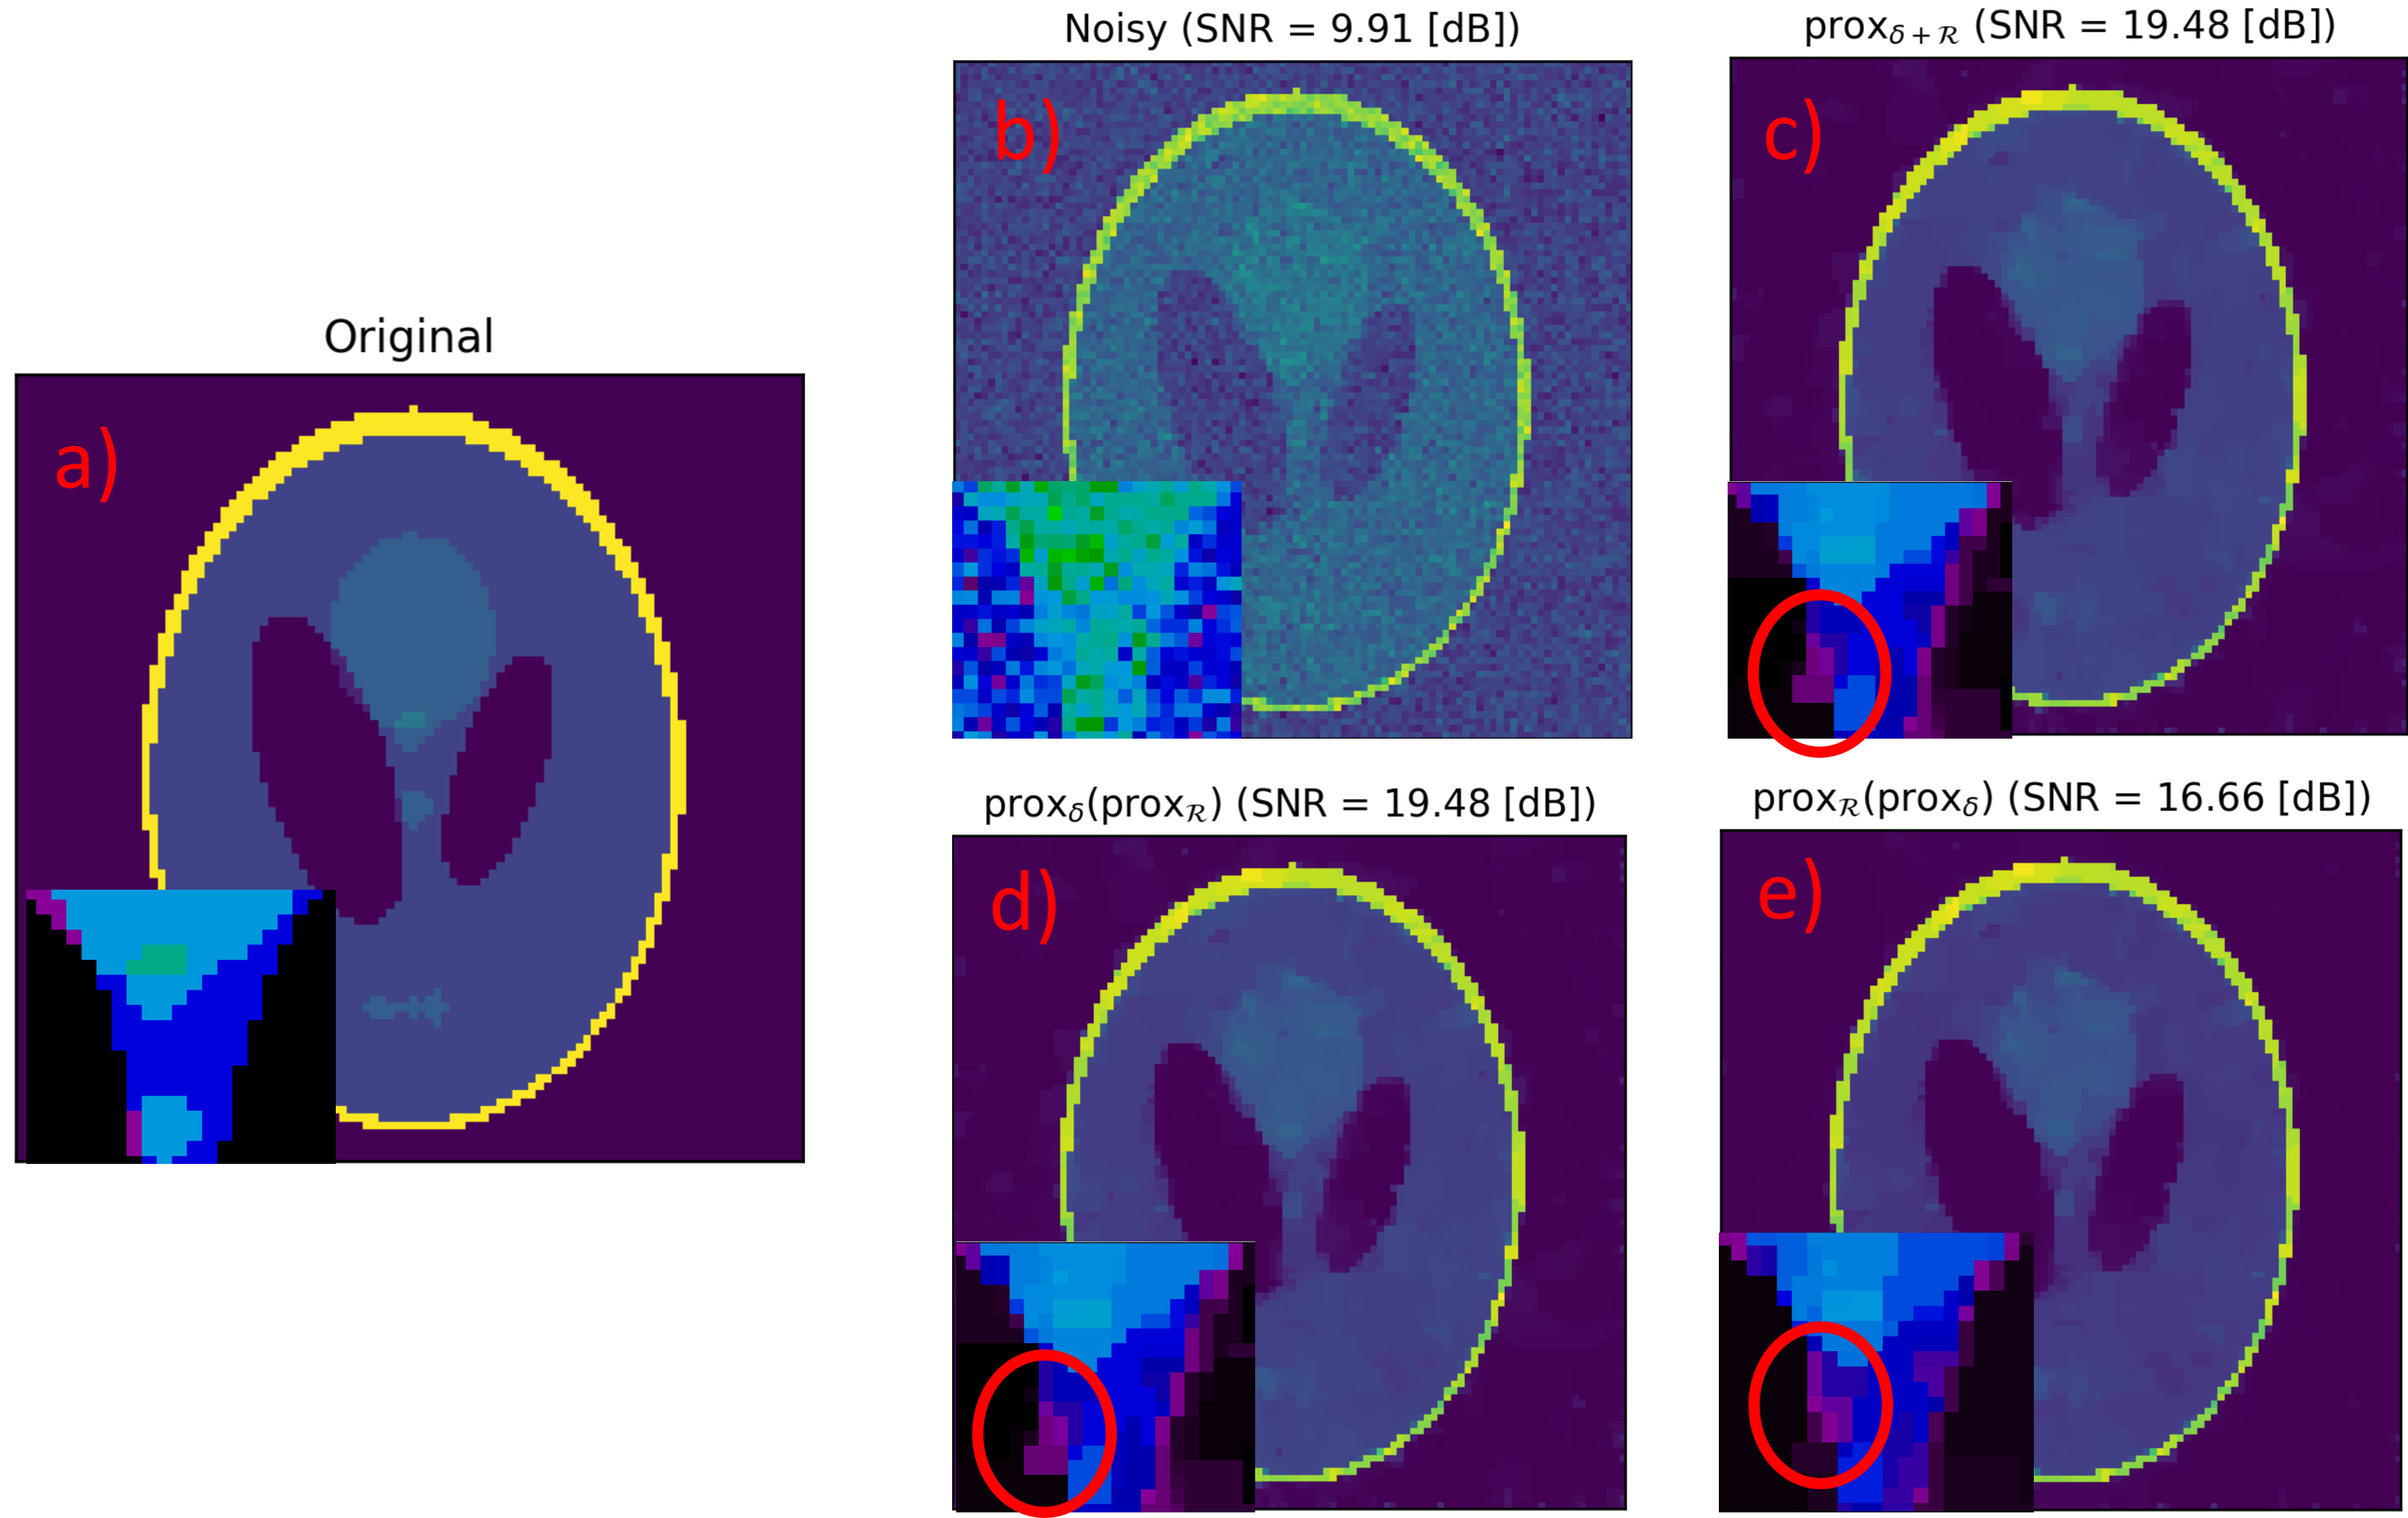
\includegraphics[scale = 0.6]{images/TV_experiments.png}
  \caption{Results of Total Variaton with nonnegativity constraints regularization on the Shepp Logan Phantom with Gaussian noise. a) shows original image, b) with Gaussian noise added, c) $\mathrm{prox}_{\mathcal{R} + \delta_{\rm \mathbb{R}_+^N}}(\mathbf{v})$ (ground truth), d) $\mathrm{prox}_{\delta_{\rm \mathbb{R}_+^N}}(\mathrm{prox}_{\mathcal{R}}(\mathbf{v}))$ (found in experiments -see table \ref{tab:exp_results}- to be equal to c), and e) $\mathrm{prox}_{\mathcal{R}}(\mathrm{prox}_{\delta_{\rm \mathbb{R}_+^N}}(\mathbf{v}))$. In each of the images, the center region is zoomed-in, to show some of the errors. Moreover, the $\mathrm{SNR}$ is shown in $\operatorname{[dB]}$.}
  \label{fig:tv_experiment}
  \end{center}
\end{figure}

In Figure \ref{fig:tv_experiment} we can see \eqref{eq:prox_nonneg(prox_r)} and \eqref{eq:prox_r(prox_nonneg)} applied to a real image. The original image was set to a size of $128 \times 128$, and normalized to the range $[0, 1]$. The added noise was sampled from the distribution $\mathcal{N}(0, 0.08)$. Just as in the random array scenario (see Table \ref{tab:exp_results}), between figures \ref{fig:tv_experiment}c) and \ref{fig:tv_experiment}d) there is an average absolute error in the order of $10^{-7}$, and the maximum absolute error is in the order of $10^{-5}$. Moreover, both visual inspection (see zoomed-in region for detailed zones) and $\mathrm{SNR}$ in $\operatorname{[dB]}$ show that both results are equal (and that there are indeed some differences between \ref{fig:tv_experiment}c) and \ref{fig:tv_experiment}e)). This promising result, that to the best of our knowledge is previously unknown, encourages the investigation of a closed-form solution of $\mathrm{prox}_{\operatorname{TV} + \delta_{\rm \mathbb{R}_+^N}}(\mathbf{v})$  and $\mathrm{prox}_{\operatorname{TV}}(\mathrm{prox}_{\delta_{\rm \mathbb{R}_+^N}}(\mathbf{v}))$, as well as the use of this result in image reconstruction libraries, as it has the potential to speed up image reconstruction.  

\noindent\textbf{Hessian-Schatten Norm}

For evaluation of the Hessian Schatten Norm, as for the evaluation of the simple Schatten norm, the results are not compelling enough to jump to a conclusion, and further investigation is required. Moreover, there are several technical constraints that hinder the proper evaluation of the Hessian Schatten Norm using CVXPy. As aforementioned, larger arrays with a higher $\sigma$ seem to have slightly more exact results, but the computational requirements of evaluating the Hessian-Schatten Norm make it unfeasible to evaluate bigger arrays than the ones presented in table \ref{tab:exp_results}. So while the results presented do not completely rule out the Hessian-Schatten norm for reduced splitting, a more efficient evaluation of the proximal operator of the Hessian-Schatten norm with nonnegativity constraints (an evaluation of the Hessian Schatten norm is presented in \cite{lefkimmiatis_poisson_2013}) is required to test for reduced splitting. 

For further evaluation, I performed an experiment on the standard test image \texttt{peppers}. The image was first normalized to the range $[0, 1]$, transformed to have a size of $64\times 64$ and finally had Gaussian noise added, sampled from $\mathcal{N}(0, 0.1)$. Regularization was done with $p=1$, which is the nuclear norm. The results are shown on figure \ref{fig:hs_experiment}
\begin{figure}[H]
  \begin{center}
  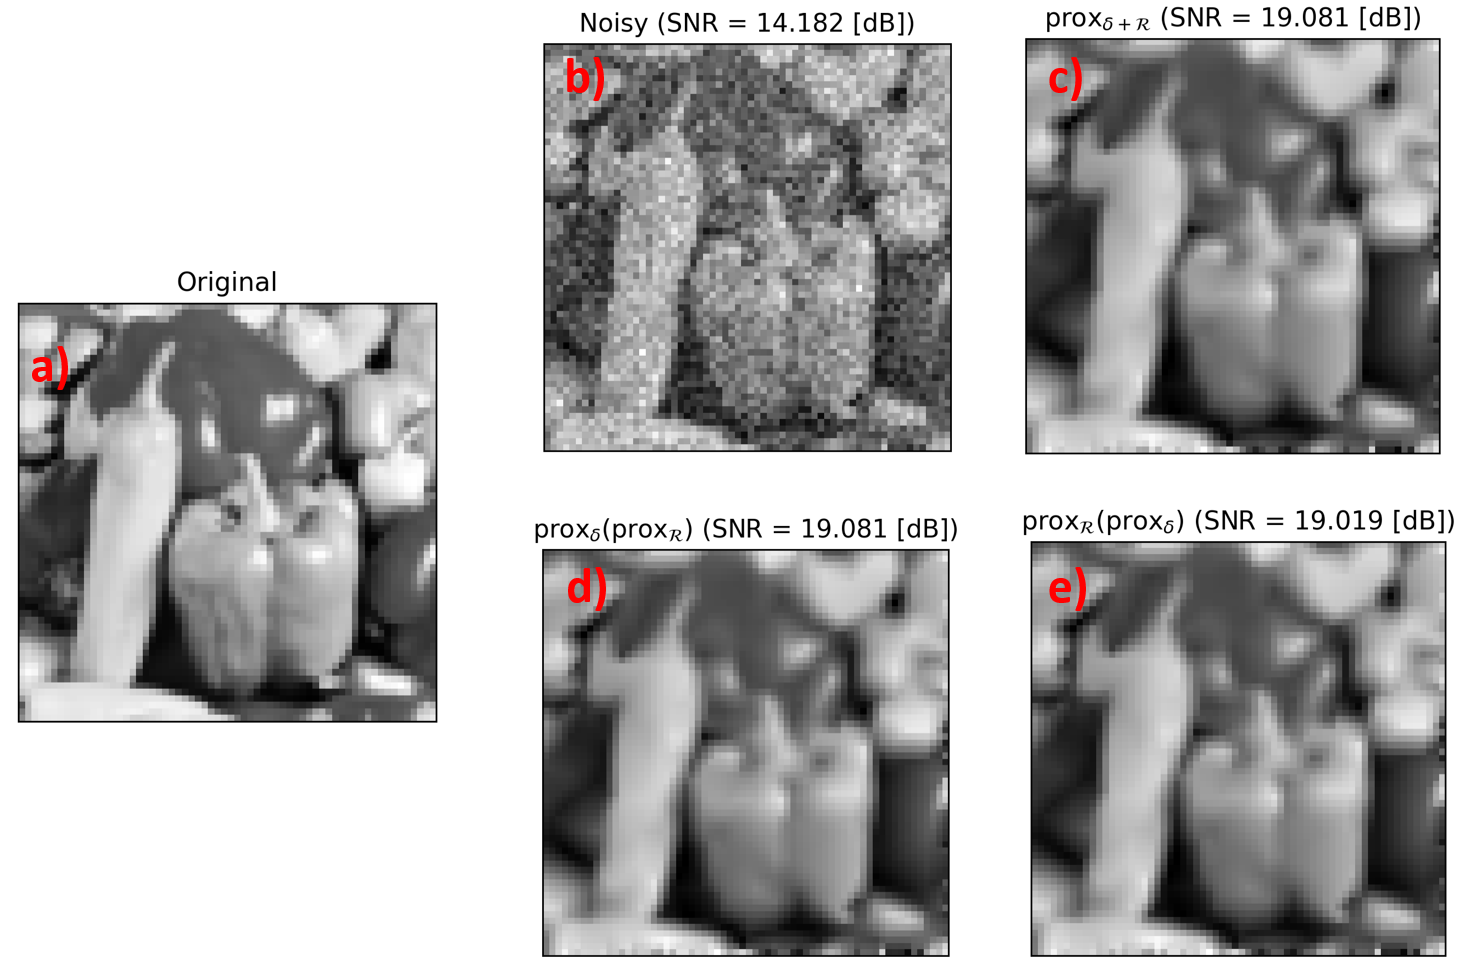
\includegraphics[scale = 0.6]{images/Peppers_experiment.png}
  \caption{Results of Hessian-Schatten norm with nonnegativity constraints regularization on standard \textit{Peppers} image with added Gaussian noise. a) shows original image in the range $[0, 1]$, b) with Gaussian noise added, sampled from $\mathcal{N}(0, 0.1)$, c) $\mathrm{prox}_{\mathcal{R} + \delta_{\rm \mathbb{R}_+^N}}(\mathbf{v})$ (ground truth), d) $\mathrm{prox}_{\delta_{\rm \mathbb{R}_+^N}}(\mathrm{prox}_{\mathcal{R}}(\mathbf{v}))$, and e) $\mathrm{prox}_{\mathcal{R}}(\mathrm{prox}_{\delta_{\rm \mathbb{R}_+^N}}(\mathbf{v}))$. Moreover, the \textit{SNR} is shown in \textit{dB}.}
  \label{fig:hs_experiment}
  \end{center}
\end{figure}

The results of the experiment on a standard test image, shown on Figure \ref{fig:hs_experiment} show the effectiveness of Hessian-Schatten norm regularization for denoising. Moreover, the experiment encourages the investigation of equation \eqref{eq:prox_nonneg(prox_r)}, as the maximum error between images \ref{fig:hs_experiment}c) and \ref{fig:hs_experiment}d) -that is, the left-hand and right-hand sides of \eqref{eq:prox_nonneg(prox_r)}- is in the order of $10^{-6}$, and the \textit{SNR} in $[\mathrm{dB}]$ is the same up to the $6^{\mathrm{th}}$ digit. On the other hand, the maximum error between images \ref{fig:hs_experiment}c) and \ref{fig:hs_experiment}e) is in the order of $10^{-2}$. While this error is not highly visible in the image, it does rule out \eqref{eq:prox_r(prox_nonneg)}. 

While the results of the experiment are encouraging, they are by no means compelling enough, as this experiment is just $1$, out of the $100$ (sampled from different distributions) that are used for the results presented in table \ref{tab:exp_results}. For further exploration, the same kind of experiment can be carried out by evaluating the proximal operator of the regularizer, instead of using a numerical approximation, as done here.  

% \newpage
\section{Conclusion} \label{sect:Conclusion}
In this project I have presented a thorough study of the combination of the proximal operator of common image regularizers with nonnegativity constraints. This is of interest because current algorithms of choice like ADMM perform variable splitting, which has a heavy computational cost. Therefore a good combination can reduce the computational load of state-of-the-art image reconstruction techniques. 

Specifically, my experimental results suggest that all the family of norms $\|\cdot\|_p$ and $\|\cdot\|_p^p$ combine well with nonnegativity constraints, a result of interest in the domains of signal and image reconstructions. Furthermore, I found that group sparsity -or the $\|\cdot\|_{p, q}$ mixed-norm- also has good combination, as all studied cases comply with  \eqref{eq:prox_r(prox_nonneg)}. In the case of more complex image regularizers, I have found that nonisotropic $\operatorname{TV}$ combines well with nonnegativity constraints. Finally, I studied the Hessian-Schatten norm, and while the result was not compelling enough to jump to a conclusion, it is promising enough to further investigate the topic.

% Specifically, I showed -in an experimental setting- how all the family of norms $\ell_p$ and $\ell_p^p$ combine well with nonnegativity constraints, a result of interest in the domains of signal and image reconstructions. Furthermore, I found that group sparsity -or the $\ell_p, \ell_q$ mixed-norm- also has good combination, as all studied cases comply with  \eqref{eq:prox_r(prox_nonneg)}. In the case of more complex image regularizers, I have found that non-isometric $\operatorname{TV}$ combines well with nonnegativity constraints. Finally, I studied the Hessian-Schatten norm, and while the result was not compelling enough to jump to a conclusion, it is promising enough to further investigate the topic. 

All of these cases are of interest because they can have a substantial effect on the performance of image reconstruction methods, and they are all commonly used regularizers. The next step is to prove the results found here using closed-form solutions, though it is out of the scope of this project. Moreover, as further work and before proving the results for closed form solutions, direct testing in an optimization library could be made. This would also allow testing on more varied settings, and images of different kinds.

\section{Acknowledgements} \label{sect:acknowledgements}
I would like to thank my supervisor, Dr. Pol del Aguila Pla, for constantly solving all kinds of doubts, from technical to theoretical. I also want to thank Pakshal Bohra, who provided me with MATLAB code to perform a similar $1$-dimensional $\operatorname{TV}$ experiment. Finally, from EPFL´s Biomedical Imaging Group, I would like to thank Thomas Debarre, and Prof. Michael Unser for fruitful discussions and feedback on the project.

% \input{for_equations}

% \newpage
% \section{Conclusion}

% Appendices
\newpage






% ------------------------------------------------------------------
% Bibliography
\bibliographystyle{ieeetr}
\bibliography{bibliography} 
% \printbibliography
% \LaTeX{} \cite{latex2e}
% \bibliographystyle{plain} % We choose the "plain" reference style
% \bibliography{bibliography} % Entries are in the "refs.bib" file
% \begin{thebibliography}{}

% \end{thebibliography}
% ------------------------------------------------------------------
% \newpage
% \begin{appendices}
% \section{GitHub Repository}
All the Jupyter notebooks, Python modules, and code in general that was used to generate the results presented in this report can be found in the Github repository \textit{Alejandro-1996/ProximalOperatorsProject} (\href{https://github.com/Alejandro-1996/ProximalOperatorsProject}{link here}).
% \end{appendices}

\end{document}